\documentclass[a4paper,12pt]{book}
\usepackage{inputenc}
\usepackage[spanish]{babel}
%\usepackage{graphicx}
\usepackage{fontspec}
%\usepackage{classicthesis} 
%\usepackage{arsclassica}
\usepackage[hidelinks]{hyperref}
%\usepackage{bookmark}
\usepackage[table]{xcolor}
\usepackage{float}
\usepackage{apacite}

\definecolor{lightgray}{gray}{0.9}
\setmainfont{Helvetica Neue}


\begin{document}

\author{Rub\'{e}n Agudo Santos}
\title{Trabajo de Fin de Grado}
\date{\today}

\frontmatter
\maketitle
\tableofcontents

\mainmatter

   \chapter{Introducci\'{o}n} 
%\newpage
El Trabajo de Fin de Grado (a partir de ahora TFG) aqu\'{i} presentado fue propuesto por un profesor de la universidad.
Las razones de la aceptaci\'{o}n del TFG fueron que se ve\'{i}a una continuidad, es decir, que se pod\'{i}a 
utilizar el TFG como entrada a un grupo de investigaci\'{o}n y/o continuar con el trabajo durante un m\'{a}ster.

\section{Planteamiento del problema}
El problema que el software ULISES, dise\~nado por el grupo de investigaci\'on GaLan en colaboraci\'on
con la universidad de Navarra, intenta resolver, es ense\~nar a alumnos habilidades. Es decir, ayudar a 
instruir a las personas cosas que no son f\'acilmente evaluables mediante un examen escrito.

ULISES es una metodolog\'ia que permite unir un sistema interactivo que exista
con un sistema educativo que tambi\'en exista para poder evaluar la realizaci\'on de tareas procedimentales 
o la adquisici\'on de habilidades.

Un ejemplo de aplicaci\'on de ULISES es el software INTRASIM 
\footnote{\url{http://www.ceit.es/index.php?option=com_content&view=article&id=112&Itemid=132}}, 
en el cual el sistema interactivo es un simulador de camiones y el sistema educativo es un software
llamado DETECTIVE.

Los datos capturados en bruto, es decir, las se\~nales generadas por el sistema de 
realidad virtual son trasladados a objetos del propio software,
que son las Observaciones y las Propiedades.

De manera resumida, una Observaci\'on es un hecho interesante en el sistema y que quiere ser observado, y 
est\'a compuesta por propiedades, que son las caracter\'isticas que la definen. En el 
apartado de Antecedentes todo se explicar\'a con mayor detalle, aqu\'i solo se pretende rascar la superficie para 
conseguir una idea general.

Una vez creadas las observaciones con sus propiedades, se crean Situaciones y Pasos. Siendo una Situaci\'on el contexto
en el que suceden las observaciones, y los Pasos c\'omo se comportan ciertas observaciones en el tiempo.

Finalmente, con esos Pasos y Situaciones el sistema, mediante distintas t\'ecnicas de diagn\'ostico 
es capaz de dar un veredicto
a la habilidad que se quiere aprender, e indic\'andole qu\'e ha hecho mal.

\section{Justificaci\'{o}n y prop\'osito}
Actualmente, la selecci\'on de pasos y situaciones se hace manualmente y con un gran componente de intuici\'on,
por lo que se hace evidente la necesidad de un software para facilitar la creaci\'on de Pasos y Situaciones porque
no es una tarea trivial. La creaci\'on de relaciones puede ser muy compleja, y el software MIPS desarrollado
en este TFG
tiene como objetivo simplificar en la medida de lo posible esa tarea, aprovechando al m\'aximo las capacidades
cognitivas del cerebro humano para identificar
patrones complejos. 

Pese a visualizarse gr\'aficamente, la identificaci\'on de esos patrones sigue sin ser algo sencillo. Es
por ello que la tarea principal del software es facilitar la identificaci\'on de intervalos donde se producen los
pasos y situaciones para posteriormente extraer de manera semiautom\'atica las relaciones entre las observaciones y
propiedades que forman parte de cada paso o situaci\'on. Esos pasos y situaciones vienen identificados por el
experto en el dominio que es quien identifica que hechos son relevantes, por ejemplo
``levantar brazo".

\section{Definiciones, acr\'{o}nimos y abreviaturas}
\textbf{TFG:} Trabajo de fin de grado.

\textbf{BD:} Base de datos.

\textbf{CVS:} Control Version System.

\textbf{MVVM:} Model-View-ViewModel.

\textbf{UI:} User Interface. Interfaz de usuario.

\textbf{MVC:} Model-view-controller.

\textbf{IDE:} Integrated Development Environment. Entorno de desarrollo integrado.

\textbf{W3C:} World Wide Web Consortium.
 
%Descripción y situación del trabajo, razones de elección del TFG, 
%planteamiento del problema y justificación del TFG 
   \chapter{Objetivos del proyecto}

%\newpage
%Objetivos, alcance, planificación temporal, herramientas, 
%gestión de riesgos, evaluación económica

\section{Objetivos}
Los objetivos del proyecto consisten en crear un software que extienda la funcionalidad actual del sistema INTRASIM desarrollado 
por la universidad de Navarra y del grupo de investigación GALAN perteneciente a la UPV/EHU.

Es un software que permite gráficamente visualizar las observaciones \footnote{Aquí va una explicación de lo que es una observación} del sistema.
El objetivo principal es brindar al experto una herramienta para poder señalar gráficamente en que momento de esa 
observación sucede el hecho concreto que estaban buscando.

La herramienta permite visualizar los datos en bruto tanto en modo v\'{i}deo (si esta disponible), como en modo gr\'{a}fico, con polilineas, histogramas etc. Tales gráficos permiten la selección de rangos.

\section{Alcance}
El alcance del proyecto se define mediante una Estructura de Descomposición del Trabajo. Es una figura en la que de manera jer\'{a}rquica
se representa que es lo que va a hacerse.
\begin{figure}[H]
    \centering
    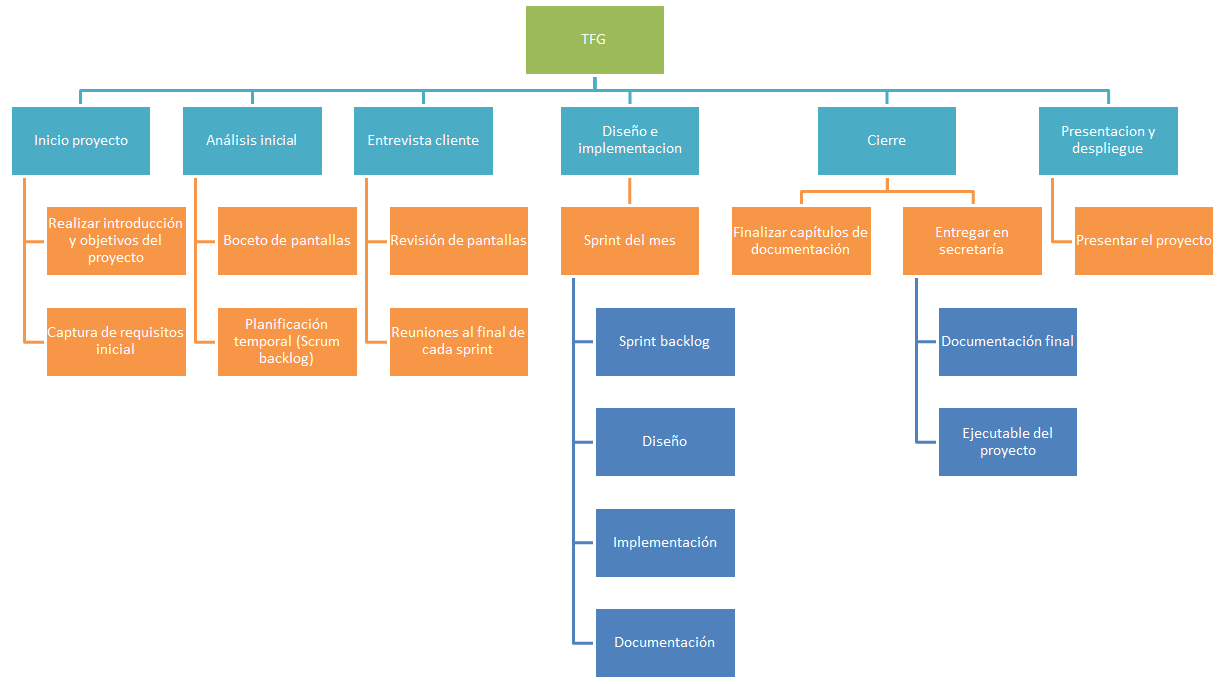
\includegraphics[width=1\linewidth]{./Figures/EDT}
    \caption[Alcance del proyecto]{EDT}
    \label{fig:Alcance}
\end{figure}

\subsection{An\'{a}lisis inicial}
\subsubsection{Boceto de pantallas}
\begin{table}[H]
    \begin{center}
        \rowcolors{1}{lightgray}{} %\rowcolors{<starting row index>}{<odd row color>}{<even row color>}
        \begin{tabular}{l p{8cm}}
            Responsable                           & Rub\'{e}n \\
            Duraci\'{o}n (horas)                  & 4. \\ 
            Esfuerzo (Horas / Persona)            & 2. \\
            Descripci\'{o}n                       & Diseño de pantallas inicial en base a las ideas obtenidas de lo
                                                    contado por Mikel, a fin de obtener dudas sobre funcionalidades. \\
            Entradas                              & Ninguna \\
            Salidas / Entregables                 & Boceto dibujado a mano con el dise\~{n}o de las pantallas \\
            Recursos necesarios                   & Papel y l\'{a}piz \\
            Precedencias                          & Ninguna \\
        \end{tabular}
    \end{center}
            
\end{table}

\subsubsection{Planificaci\'{o}n temporal (Scrum Backlog)}
\begin{table}[H]
    \begin{center}
        \rowcolors{1}{lightgray}{} %\rowcolors{<starting row index>}{<odd row color>}{<even row color>}
        \begin{tabular}{l p{8cm}}
            Responsable                           & Rub\'{e}n \\
            Duraci\'{o}n (horas)                  & 7. \\ 
            Esfuerzo (Horas / Persona)            & 7. \\
            Descripci\'{o}n                       & Creacion de cada sprint con sus respectivas tareas para crear la pila de tareas. \\
            Entradas                              & Requisitos del cliente.\\
            Salidas / Entregables                 & Un listado con todas las tareas a completar \\
            Recursos necesarios                   & PC con un editor de textos.\\
            Precedencias                          & Requisitos del cliente. \\
        \end{tabular}
    \end{center}
    
\end{table}

\subsubsection{Realizar introducci\'{o}n y objetivos del proyecto}
\begin{table}[H]
    \begin{center}
        \rowcolors{1}{lightgray}{} %\rowcolors{<starting row index>}{<odd row color>}{<even row color>}
        \begin{tabular}{l p{8cm}}
            Responsable                           & Rub\'{e}n \\
            Duraci\'{o}n                          & 7. \\ 
            Esfuerzo (Horas / Persona)            & 7. \\
            Descripci\'{o}n                       & Realizar las secciones de la memoria de la Introducci\'{o}n y los
                                                    objetivos del proyecto. \\
            Entradas                              & Scrum backlog  \\
            Salidas / Entregables                 & Los cap\'{i}tulos de introducci\'{o}n y objetivos del proyecto. \\
            Recursos necesarios                   & PC, \LaTeX, TeXStudio, Scrum backlog \\
            Precedencias                          & Scrum backlog. \\
        \end{tabular}
    \end{center}
    
\end{table}

\subsection{Entrevista cliente}
\subsubsection{Revisi\'{o}n de pantallas}
\begin{table}[H]
    \begin{center}
        \rowcolors{1}{lightgray}{} %\rowcolors{<starting row index>}{<odd row color>}{<even row color>}
        \begin{tabular}{l p{8cm}}
            Responsable                           & Rub\'{e}n \\
            Duraci\'{o}n                          & 2. \\ 
            Esfuerzo (Horas / Persona)            & 1.5 \\
            Descripci\'{o}n                       & Mostrar al cliente (Mikel), un prototipo inicial de pantallas
                                                    para asi poder mejorar el dise\~{n}o para que sea mas f\'{a}cil de usar. \\
            Entradas                              & Requisitos del cliente. \\
            Salidas / Entregables                 & Prototipo realizado en WPF que muestra el comportamiento y forma de las pantallas. \\
            Recursos necesarios                   & Visual Studio 2013, Avalon Dock, un PC. \\
            Precedencias                          & Captura de requisitos inicial. \\
        \end{tabular}
    \end{center}
    
\end{table}

\subsubsection{Reuniones al final de cada sprint}
\begin{table}[H]
    \begin{center}
        \rowcolors{1}{lightgray}{} %\rowcolors{<starting row index>}{<odd row color>}{<even row color>}
        \begin{tabular}{l p{8cm}}
            Responsable                           & Rub\'{e}n \\
            Duraci\'{o}n                          & 2. \\ 
            Esfuerzo (Horas / Persona)            & 1.5 \\
            Descripci\'{o}n                       & Reuni\'{o}n para que el director de proyecto vea como va el trabajo,
                                                    aclarar dudas etc. \\
            Entradas                              & El trabajo realizado hasta el momento.\\
            Salidas / Entregables                 & Ninguno / acta de reuni\'{o}n \\
            Recursos necesarios                   & PC con el programa funcional. \\
            Precedencias                          & Ninguno. \\
        \end{tabular}
    \end{center}
    
\end{table}

\subsection{Dise\~{n}o e implementaci\'{o}n}
\subsubsection{Sprint backlog}
\begin{table}[H]
    \begin{center}
        \rowcolors{1}{lightgray}{} %\rowcolors{<starting row index>}{<odd row color>}{<even row color>}
        \begin{tabular}{l p{8cm}}
            Responsable                           & Rub\'{e}n \\
            Duraci\'{o}n                          & 1 \\ 
            Esfuerzo (Horas / Persona)            & 0.5 \\
            Descripci\'{o}n                       & Elegir las tareas que van a conformar el sprint del mes. \\
            Entradas                              & La lista de tareas completa\\
            Salidas / Entregables                 & Post-it con las tareas seleccionadas para ese sprint \\
            Recursos necesarios                   & Post-it, boli y lista de tareas. \\
            Precedencias                          & Scrum backlog \\
        \end{tabular}
    \end{center}
    
\end{table}

\subsubsection{Dise\~{n}o}
\begin{table}[H]
    \begin{center}
        \rowcolors{1}{lightgray}{} %\rowcolors{<starting row index>}{<odd row color>}{<even row color>}
        \begin{tabular}{l p{8cm}}
            Responsable                           & Rub\'{e}n \\
            Duraci\'{o}n                          & 10. \\ 
            Esfuerzo (Horas / Persona)            & 4. \\
            Descripci\'{o}n                       & Realizar el diseño de software, clases, Interfaces necesarias, que patrones van a usarse etc. \\
            Entradas                              & Tarea a realizar y la interfaz de usuario.\\
            Salidas / Entregables                 & Dise\~{n}o de software que guiar\'{a} la siguiente tarea y la documentaci\'{o}n
                                                    habr\'{a} sido actualizada en consecuencia. \\
            Recursos necesarios                   & La documentaci\'{o}n realizada hasta el momento, Visual Studio 2013, Git y un PC. \\
            Precedencias                          & Sprint Backlog. \\
        \end{tabular}
    \end{center}
    
\end{table}

\subsubsection{Implementaci\'{o}n}
\begin{table}[H]
    \begin{center}
        \rowcolors{1}{lightgray}{} %\rowcolors{<starting row index>}{<odd row color>}{<even row color>}
        \begin{tabular}{l p{8cm}}
            Responsable                           & Rub\'{e}n \\
            Duraci\'{o}n                          & 20. \\ 
            Esfuerzo (Horas / Persona)            & 20. \\
            Descripci\'{o}n                       & Implementar lo dise\~{n}ado, lo que describe la tarea en el post-it del sprint. \\
            Entradas                              & Dise\~{n}o realizado sobre la tarea, post-it con la tarea.\\
            Salidas / Entregables                 & La pieza de software con la nueva funcionalidad implementada, y la documentaci\'{o}n
                                                    actualizada. \\
            Recursos necesarios                   & La documentaci\'{o}n realizada hasta el momento, Visual Studio 2013, Git y un PC. \\
            Precedencias                          & Dise\~{n}o. \\
        \end{tabular}
    \end{center}
    
\end{table}

\subsubsection{Documentaci\'{o}n}
\begin{table}[H]
    \begin{center}
        \rowcolors{1}{lightgray}{} %\rowcolors{<starting row index>}{<odd row color>}{<even row color>}
        \begin{tabular}{l p{8cm}}
            Responsable                           & Rub\'{e}n \\
            Duraci\'{o}n                          & 10. \\ 
            Esfuerzo (Horas / Persona)            & 5. \\
            Descripci\'{o}n                       & Revisar y actualizar la documentaci\'{o}n realizada durante el sprint. \\
            Entradas                              & La documentaci\'{o}n realizada hasta el momento.\\
            Salidas / Entregables                 & La documentaci\'{o}n actualizada. \\
            Recursos necesarios                   & La documentaci\'{o}n. \\
            Precedencias                          & Implementaci\'{o}n. \\
        \end{tabular}
    \end{center}
    
\end{table}

\subsection{Cierre}
\subsubsection{Finalizar cap\'{i}tulos de documentaci\'{o}n}
\begin{table}[H]
    \begin{center}
        \rowcolors{1}{lightgray}{} %\rowcolors{<starting row index>}{<odd row color>}{<even row color>}
        \begin{tabular}{l p{8cm}}
            Responsable                           & Rub\'{e}n \\
            Duraci\'{o}n                          & 30. \\ 
            Esfuerzo (Horas / Persona)            & 30. \\
            Descripci\'{o}n                       & Realizar los cap\'{i}tulos adicionales: Verificaci\'{o}n y evaluaci\'{o}n, conclusiones y trabajo futuro
                                                    etc. \\
            Entradas                              & La documentaci\'{o}n realizada. \\
            Salidas / Entregables                 & La documentaci\'{o}n terminada. \\
            Recursos necesarios                   & \LaTeX, Git, y un PC. \\
            Precedencias                          & Dise\~{n}o e implementaci\'{o}n (categor\'{i}a). \\
        \end{tabular}
    \end{center}
    
\end{table}

\subsubsection{Documentaci\'{o}n final}
\begin{table}[H]
    \begin{center}
        \rowcolors{1}{lightgray}{} %\rowcolors{<starting row index>}{<odd row color>}{<even row color>}
        \begin{tabular}{l p{8cm}}
            Responsable                           & Rub\'{e}n \\
            Duraci\'{o}n                          & 1 \\ 
            Esfuerzo (Horas / Persona)            & 1 \\
            Descripci\'{o}n                       & Entregar la documentaci\'{o}n en secretar\'{i}a \\
            Entradas                              & La documentaci\'{o}n. \\
            Salidas / Entregables                 & Ninguna. \\
            Recursos necesarios                   & La documentaci\'{o}n impresa. \\
            Precedencias                          & Finalizar cap\'{i}tulos de la documentaci\'{o}n. \\
        \end{tabular}
    \end{center}
    
\end{table}

\subsubsection{Ejecutable del proyecto}
\begin{table}[H]
    \begin{center}
        \rowcolors{1}{lightgray}{} %\rowcolors{<starting row index>}{<odd row color>}{<even row color>}
        \begin{tabular}{l p{8cm}}
            Responsable                           & Rub\'{e}n \\
            Duraci\'{o}n                          & 1. \\ 
            Esfuerzo (Horas / Persona)            & 1. \\
            Descripci\'{o}n                       & Entregar un CD con el ejecutable del proyecto realizado. \\
            Entradas                              & El c\'{o}digo fuente del programa. \\
            Salidas / Entregables                 & El ejecutable binario y el CD con el software. \\
            Recursos necesarios                   & PC con grabadora, y un CD grabable en blanco. \\
            Precedencias                          & Finalizar cap\'{i}tulos de la documentaci\'{o}n. \\
        \end{tabular}
    \end{center}
    
\end{table}

\subsection{Presentaci\'{o}n y despliegue}
\subsubsection{Presentar el proyecto}
\begin{table}[H]
    \begin{center}
        \rowcolors{1}{lightgray}{} %\rowcolors{<starting row index>}{<odd row color>}{<even row color>}
        \begin{tabular}{l p{8cm}}
            Responsable                           & Rub\'{e}n \\
            Duraci\'{o}n                          & 20 minutos. \\ 
            Esfuerzo (Horas / Persona)            & 20 minutos. \\
            Descripci\'{o}n                       & Presentar el proyecto y defenderlo ante el tribunal. \\
            Entradas                              & Slides de la presentaci\'{o}n.\\
            Salidas / Entregables                 & Ninguna. \\
            Recursos necesarios                   & PC con LibreOffice Impress. \\
            Precedencias                          & Categor\'{i}a cierre. \\
        \end{tabular}
    \end{center}
    
\end{table}


\section{Planificaci\'{o}n temporal}
En vez de seguir una planificación clásica, como puede ser COCOMO \footnote{\url{http://sunset.usc.edu/csse/research/COCOMOII/cocomo_main.html}} o Waterfall \footnote{\url{http://pdf.aminer.org/000/361/405/software_requirements_are_they_really_a_problem.pdf}} he decidido utilizar las metodologías agiles de desarrollo, concretamente Scrum y Kanban

\subsection{Scrum}
Scrum es una serie de herramientas (framework) para la gestión y desarrollo de software basado en un proceso iterativo e incremental. \emph{cita a la wikipedia}

\begin{figure}[H]
    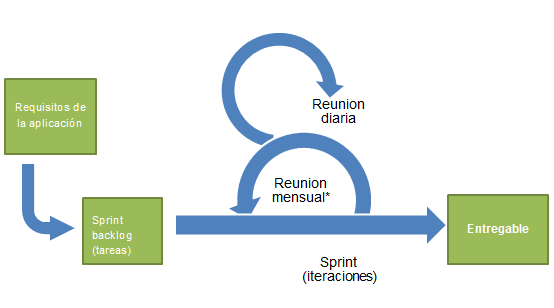
\includegraphics[width=0.7\linewidth]{./Figures/Scrumm}
    \caption[Proceso iterativo Scrum]{En este gráfico podemos ver el método de trabajo según Scrum, en el cual se observa lo importante que son los entregables}
    \label{fig:Scrum}
\end{figure}



%\newpage
Scrum, de manera resumida consiste en lo siguiente:
\begin{enumerate}
    \item Hablar con el cliente para ver si hay nuevos requisitos.
    \item Crear backlog, es decir, las tareas de ese sprint.
    \item Programar los requisitos especificados en el sprint.
    \item Reunión de retrospectiva para ver que ha ido mal y mejorarlo.
    \item Enviar entregable al cliente.
    \item Repetir.
\end{enumerate}

Es fundamental entre sprint y sprint que el valor del producto haya aumentado. Es decir, lo importante es el producto, no como vamos nosotros en el propio proyecto. Podríamos haber avanzado mucho en el diseño del software, pero si eso es algo que el cliente no puede ver estaremos fallando en nuestra agilidad.

Por otro lado, si cometemos algún error será muy sencillo corregir el error ya que si los sprints son de dos semanas por ejemplo, no habremos perdido apenas tiempo. Y además para el cliente los entregables serán predecibles en el tiempo.

Scrum es también muy importante, y se posiciona como una alternativa muy potente frente a COCOMO o waterfall, es porque en la creación de software hay un componente de incertidumbre muy grande. No sabemos como, ni cuando pueden cambiar los requisitos de un software. Por ello toman importancia los sprints de nuevo. 

En los modelos antiguos, si ya habíamos terminado la fase de análisis y diseño, y se requería una nueva funcionalidad es necesario paralizar el desarrollo del software y volver a analizar y diseñar. En cambio, con Scrum es posible integrar ese cambio en el siguiente sprint.

\subsection{Kanban}
Kanban es un método de organización del conocimiento del trabajo que se está realizando con un gran énfasis en el la entrega justo a tiempo \footnote{JIT Delivery: Just-In-Time Delivery} sin sobrecargar al equipo \emph{Cita a la wikipedia}

Kanban se centra mucho en que lo importante no es empezar muchas cosas, si no que acabemos aquello que empezamos. Sirve sobre todo para ver de una manera visual:
\begin{itemize}
    \item Qué tenemos pendiente
    \item Qué estamos haciendo ahora mismo
    \item Qué hemos terminado.
\end{itemize}

El método Kanban es algo muy extenso, pero yo simplemente he aplicado el tablero Kanban mezclado con Scrum. Cada dos semanas, me creo una lista de tareas que debo completar (Backlog) y lo coloco en la columna de "Tareas pendientes", ordenadas por prioridad. Después, coloco en la lista de "En progreso" como máximo dos tareas. Y no empiezo ninguna otra hasta que esas dos hayan sido pasadas a la columna de "Tareas finalizadas".

\subsection{Mi planificaci\'{o}n}
Cada sprint tiene una duraci\'{o}n de un mes, empezando desde Septiembre del 2013.
\subsubsection{Sprint 1}
Este sprint era el comienzo del proyecto, establecer prioridades, documentarse etc. Lo que ha compuesto este sprint ha sido:

\begin{itemize}
    \item Crear y configurar el repositorio Git y los clientes en los dos ordenadores.
    \item Leer la documentaci\'{o}n existente y obtener el c\'{o}digo fuente original.
    \item Iniciar dise\~{n}os gr\'{a}ficos preliminares en papel para elegir las librer\'{i}as necesarias.
    \item Buscar y documentarse sobre las librer\'{i}as que cumplan los requisitos del punto anterior. 
\end{itemize} 

\subsubsection{Sprint 2}
Una vez configurado y elegidas las librer\'{a}s necesarias lo siguiente que se hizo fue:

\begin{itemize}
    \item Reunirse con Mikel para realizar una captura de requisitos.
    \item Dise\~{n}ar unos prototipos funcionales.
    \item Documentar lo que se hab\'{i}a realizado hasta el momento, es decir, el tipo de planificaci\'{o}n que se hab\'{i}a elegido,
    tecnolog\'{i}as que se iban a usar etc.
\end{itemize}

\subsubsection{Sprint 3}
El siguiente paso consiste en poder cargar v\'{i}deos, tantos como se quieran, desde el sistema de archivos.

\begin{itemize}
    \item Crear el control de cargar v\'{i}deos (contenedor de v\'{i}deos). El contenedor debe permitir:
    \begin{itemize}
        \item Cargar distintos v\'{i}deos desde el sistema de archivos.
        \item Cada v\'{i}deo debe disponer de sus controles individuales. Play, pausa, stop y avanzar de tantos segundos en tantos segundos, y que sea
        configurable por el usuario, mediante un archivo de configuraci\'{o}n.
        \item El contenedor de v\'{i}deos debe tener de unos controles generales que pause, y que los reproduzca de manera simultanea
        para mantener la sincronizaci\'{o}n.
        \item Debe permitir establecer para cada v\'{i}deo el momento de inicio del v\'{i}deo manualmente para mantener la sincronizaci\'{o}n.
    \end{itemize}
\end{itemize}

\subsubsection{Sprint 4}
Despu\'{e}s de terminar la visualizaci\'{o}n de v\'{i}deos, lo siguiente en la lista de tareas es crear un visualizador de datos.

\begin{itemize}
    \item Crear el contenedor que nos permita visualizar datos. El control debe permitir:
    \begin{itemize}
        \item Visualizar datos continuos y discretos.
        \item Seleccionar un rango en la gr\'{a}fica, estableciendo un inicio y un fin para un paso.
        \item Que muestre el progreso, y que este sincronizado con el v\'{i}deo.
        \item Guardar el inicio y fin del paso en la base de datos.
        
    \end{itemize}
\end{itemize}

\subsubsection{Sprint 5}
Ya tenemos todo preparado para funcionar, ahora hay que poder guardar datos.

\begin{itemize}
    \item Elegir una Base de Datos.
    \item Configurar los usuarios y permisos de la base de datos.
    \item Crear el diagrama Entidad-Relaci\'{o}n que representara el modo de guardado de datos.
    \item A\~{n}adir al c\'{o}digo existente las llamadas necesarias a la base de datos.
    \item Permitir cambiar la ubicaci\'{o}n de la base de datos mediante un archivo de configuraci\'{o}n.
\end{itemize}

\subsubsection{Sprint 6}
En este momento ya tenemos una aplicaci\'{o}n completamente funcional pero con datos de prueba. Hay que poder cargar datos de los XML.

\begin{itemize}
    \item Crear la clase que lea los XML.
    \item Hablar con Mikel para saber como est\'{a}n guardadas las observaciones.
    \item Utilizando los datos del XML cargar la aplicaci\'{o}n con esos datos.
\end{itemize}

\subsubsection{Observaciones}
N\'{o}tese que hay 6 sprints y desde septiembre hasta junio hay 10 meses. Por lo que se entiende que el resto de tiempo es para:
\begin{enumerate}
    \item Poder realizar las tareas de clase.
    \item Amortiguar el impacto de los retrasos que puedan darse.
\end{enumerate}

\section{Herramientas}
El proyecto, al no ser enteramente mío, no he tenido una libertad total para la elección de herramientas. 

Las herramientas que he utilizado para llevar a cabo este proyecto han sido:
\begin{itemize}
    \item 
    \textbf{Visual Studio}
    
    Para el desarrollo propiamente dicho del proyecto he usado Visual Studio 2013 Ultimate, proporcionado de manera gratuita gracias al acuerdo que mantiene la UPV/EHU con Microsoft.
    
    \item 
    \textbf{TeXstudio y \LaTeX}
    
    Dos herramientas gratuitas y de código abierto para generar documentos.
    
    \item
    \textbf{Git y GitHub}
    
    Fundamental en los proyectos que se basen en metodologías ágiles. Git es un software de gestión de control de versiones distribuido, esto es, que cada desarrollador dispone de una copia completa del repositorio, desarrollado por Linus Torvalds y Junio Hamano en 2005 y similar a SVN.
    
    \item
    \textbf{OxyPlot}
    
    Librer\'{i}a de c\'{o}digo abierto y multiplataforma que permite crear gr\'{a}ficos de manera sencilla as\'{i} como seleccionar rangos etc.
    
\end{itemize}

\section{Gesti\'{o}n de riesgos}
Dadas las fechas de entrega impuestas por mi mismo para la finalizaci\'{o}n del Trabajo de Fin de Grado, es un hecho que
aparecerán riesgos que pueden poner en peligro el proyecto. Es por ello que se necesita tener en cuenta las probabilidades de los sucesos que 
pueden ocurrir y que puedan retrasar el trabajo de forma notable. Una vez
listados, se puede proceder a crear un plan de prevención para evitarlos. Y en caso de que la prevención no
funcionara, un plan de contingencia que pueda amortiguar las consecuencias de ese riesgo. A continuación
se listan de forma detallada los riesgos que pueden aparecer durante el transcurso del proyecto.

\subsection{Planificaci\'{o}n}
En esta categor\'{i}a se engloban los riesgos que sean causados por una mala planificaci\'{o}n temporal.
\subsubsection{Mala concepci\'{o}n del proyecto}
\begin{table}[H]
    \begin{center}
       \rowcolors{1}{lightgray}{} %\rowcolors{<starting row index>}{<odd row color>}{<even row color>}
       \begin{tabular}{l p{8cm}}
           Descripci\'{o}n                 & Por decisiones erróneas, como puede ser elegir utilizar una
           base de datos, puede que el trabajo deba ser reconstruido desde el principio. \\
           Prevenci\'{o}n                  & Una buena planificación y conocimiento exacto de lo que quiere y necesita el cliente. \\ 
           Plan de contingencia            & Un programa flexible a cambios \\
           Probabilidad                    & Improbable \\
           Impacto                         & Muy alto\\
        \end{tabular}
    \end{center}
    
\end{table}
\subsubsection{Error en la planificaci\'{o}n temporal}
\begin{table}[H]
    \begin{center}
        \rowcolors{1}{lightgray}{} %\rowcolors{<starting row index>}{<odd row color>}{<even row color>}
        \begin{tabular}{l p{8cm}}
            Descripci\'{o}n                 & Por una mala compresión y falta de experiencia el cálculo
            de tiempo estimado de una de las tareas es erróneo y hay que reajustar todo el proyecto. \\
            Prevenci\'{o}n                  & Realizar la estimación lo mejor posible y tener una buena
            comunicación con el cliente para no tener fallos de comprensión. \\ 
            Plan de contingencia            & Margen de error en los tiempos \\
            Probabilidad                    & Muy probable \\
            Impacto                         & Medio\\
        \end{tabular}
    \end{center}
    
\end{table}
\subsection{Entorno de desarrollo}
\subsubsection{Incompatibilidad de versiones}
\begin{table}[H]
    \begin{center}
        \rowcolors{1}{lightgray}{} %\rowcolors{<starting row index>}{<odd row color>}{<even row color>}
        \begin{tabular}{l p{8cm}}
            Descripci\'{o}n                 & Al utilizar dos ordenadores, una workstation y un port\'{a}til puede que no disponga de las mismas
            versiones del software o que no se satisfagan todas las dependencias. \\
            Prevenci\'{o}n                  & Asegurarme de disponer el mismo software con las mismas versiones. \\ 
            Plan de contingencia            & Resolver manualmente las dependencias. \\
            Probabilidad                    & Probable \\
            Impacto                         & Bajo\\
        \end{tabular}
    \end{center}
    
\end{table}
\subsubsection{Problemas con GIT}
\begin{table}[H]
    \begin{center}
        \rowcolors{1}{lightgray}{} %\rowcolors{<starting row index>}{<odd row color>}{<even row color>}
        \begin{tabular}{l p{8cm}}
            Descripci\'{o}n                 & Al ser algo no ense\~{n}ado en profundidad en clase puede causar problemas al usar las
            funciones avanzadas. \\
            Prevenci\'{o}n                  & Tener un buen manual y tener una copia local en otra carpeta para prevenir perdidas de informaci\'{o}n. \\ 
            Plan de contingencia            & Desechar el software de control de versiones y buscar alternativas como Dropbox. \\
            Probabilidad                    & Poco probable \\
            Impacto                         & Bajo \\
        \end{tabular}
    \end{center}  
\end{table}
\subsubsection{Problemas con las librer\'{i}as}
\begin{table}[H]
    \begin{center}
        \rowcolors{1}{lightgray}{} %\rowcolors{<starting row index>}{<odd row color>}{<even row color>}
        \begin{tabular}{l p{8cm}}
            Descripci\'{o}n                 & Que las librar\'{i}as escogidas no cumplan los requisitos necesarios \\
            Prevenci\'{o}n                  & Mirar con anterioridad que las librar\'{i}as cumplen todos nuestros requisitos. \\ 
            Plan de contingencia            & Buscar otra librar\'{i}a o intentar parchear la actual, ya que son de c\'{o}digo abierto. \\
            Probabilidad                    & Muy probable \\
            Impacto                         & Alto \\
        \end{tabular}
    \end{center}
    
\end{table}
\subsection{Usuarios finales y clientes}
\subsubsection{No agrado del producto}
\begin{table}[H]
    \begin{center}
        \rowcolors{1}{lightgray}{} %\rowcolors{<starting row index>}{<odd row color>}{<even row color>}
        \begin{tabular}{l p{8cm}}
            Descripci\'{o}n                 & Despu\'{e}s de la entrega del proyecto puede suceder que el cliente no est\'{e} satisfecho. \\
            Prevenci\'{o}n                  & Una buena comunicación con el cliente y reuniones progresivas para ir mostrando la evolución del proyecto. \\ 
            Plan de contingencia            & Blindar las caracter\'{i}sticas, solo se realizaran las estipuladas durante el proyecto. \\
            Probabilidad                    & Probable \\
            Impacto                         & Muy alto \\
        \end{tabular}
    \end{center}
    
\end{table}

\subsubsection{Manejo poco intuitivo}
\begin{table}[H]
    \begin{center}
        \rowcolors{1}{lightgray}{} %\rowcolors{<starting row index>}{<odd row color>}{<even row color>}
        \begin{tabular}{l p{8cm}}
            Descripci\'{o}n                 & Como  los  programadores  tienen  un  conocimiento
            inform\'{a}tico superior no tendr\'{a}n problemas con el uso, pero los usuarios si pueden tenerlos.\\
            Prevenci\'{o}n                  & Un diseño de interfaz sencillo y probar versiones con
            usuarios con conocimientos inform\'{a}ticos bajos. \\ 
            Plan de contingencia            & Adaptar la interfaz en el siguiente sprint. \\
            Probabilidad                    & Probable. \\
            Impacto                         & Alto \\
        \end{tabular}
    \end{center}
    
\end{table}

\subsection{Personas}
\subsubsection{Bajas por enfermedad}
\begin{table}[H]
    \begin{center}
        \rowcolors{1}{lightgray}{} %\rowcolors{<starting row index>}{<odd row color>}{<even row color>}
        \begin{tabular}{l p{8cm}}
            Descripci\'{o}n                 & El \'{u}nico componente del equipo cae enfermo y no puede trabajar. \\
            Prevenci\'{o}n                  & No existe prevenci\'{o}n. \\ 
            Plan de contingencia            & Recuperarse lo antes posible y manejar cierta holgura con las fechas.\\
            Probabilidad                    & Probable. \\
            Impacto                         & Muy alto \\
        \end{tabular}
    \end{center}
    
\end{table}

\subsection{Requisitos}
\subsubsection{Nuevos requisitos}
\begin{table}[H]
    \begin{center}
        \rowcolors{1}{lightgray}{} %\rowcolors{<starting row index>}{<odd row color>}{<even row color>}
        \begin{tabular}{l p{8cm}}
            Descripci\'{o}n                 & Debido a que el cliente tiene nuevas necesidades solicita la
            implementaci\'{o}n de funcionalidades extras o la desaparici\'{o}n de alguna que se hayan podido volver innecesarias. \\
            Prevenci\'{o}n                  & Realizar un buen dise\~{n}o para la posibilidad de añadir
            funcionalidades sin que suponga un coste muy elevado. \\ 
            Plan de contingencia            & Evaluar los nuevos requisitos para saber si se pueden
            abordar o no y si fuese que si estudiar la situación y asignar el trabajo a los trabajadores. \\
            Probabilidad                    & Probable \\
            Impacto                         & Alto \\
        \end{tabular}
    \end{center}
    
\end{table}

\subsubsection{Requisitos no contemplados (ocultos)}
\begin{table}[H]
    \begin{center}
        \rowcolors{1}{lightgray}{} %\rowcolors{<starting row index>}{<odd row color>}{<even row color>}
        \begin{tabular}{l p{8cm}}
            Descripci\'{o}n                 & Requisitos explícitos desde el principio, pero que no fueron
            vistos en el primer an\'{a}lisis y al verlos en un futuro, provocan cambios en todos los niveles. \\
            Prevenci\'{o}n                  & Utilizar correctamente Scrum. \\ 
            Plan de contingencia            & A\~{n}adirlo como una tarea al siguiente sprint. \\
            Probabilidad                    & Muy probable. \\
            Impacto                         & Medio-Bajo. \\
        \end{tabular}
    \end{center}
    
\end{table}

\section{Planificaci\'{o}n econ\'{o}mica}
No se obtendr\'{a} beneficio econ\'{o}mico del proyecto ya que se hace por el bien de la ciencia, y porque esta licenciado
bajo licencia GPLv3.

Por lo tanto el coste de venta de nuestro coste sera 0€

\subsection{Amortizaci\'{o}n de material}
\subsubsection{Oficina}
La oficina que utilizamos es el domicilio familiar y no hay que pagar alquiler ya que es de nuestra propiedad. Por lo que el gasto de alquiler/hipoteca es 0€
\subsubsection{Material inform\'{a}tico}
El material informático que se va a usar es un portátil Acer TravelMate 5742G comprado en 
Diciembre de 2010 y usado intensivamente durante estos 4 años. 
El portátil estaba pensado para ser amortizado en 4 años. \emph{As\'{i} que por aqui habra que hacer algun calculo tonto}, por lo que durante el 
transcurso del TFG no va a generar ning\'{u}n tipo de gasto.

Tambi\'{e}n se va a usar un PC gen\'{e}rico comprado a piezas en 2012.

\subsection{Otros gastos}

\begin{tabular}{l*{1}{c}r}
    Concepto                   & Gastos en € / mes & \\
    \hline
    Luz                        & 60 & \\
    Agua                       & 50 & \\
    Internet + Teléfono        & 60 & \\
    Gas                        & 70 & \\
    \hline
    Total Mes                  & 325 & \\
    Total A\~{n}o              & 3900 &\\
\end{tabular}


   \chapter{Antecedentes}

%Situación actual, estudio de diferentes alternativas 
%existentes o distintos posibles enfoques del problema a solucionar
\section{Situaci\'on actual}
El proyecto ULISES desarrollado por el grupo de investigaci\'on GaLan, en colaboraci\'on con la universidad de Navarra, 
consiste en un software que permite la integraci\'on de cualquier sistema interactivo con cualquier
sistema educativo. Es decir, sirve para ense\~nar habilidades que necesitan de un profesor experto que los eval\'ue,
ya sea en tiempo real, o a trav\'es de un v\'ideo.


La parte de los sistemas interactivos puede estar formada, por ejemplo, por un simulador de conducci\'on de camiones,
un sistema de captura de movimientos, un kinect, etc.

Por otro lado, el sistema educativo puede ser moodle, DETECTIVE o cualquier software que permita evaluar algo.

El objetivo principal es conseguir un sistema en el que la gente entrene una habilidad concreta, por ejemplo, aprender
a sacar correctamente en tenis, y que el sistema sea capaz de evaluar, determinar d\'onde se ha equivocado, y en definitiva,
ayudar a esa persona a aprender a realizar un saque de tenis correctamente.

Para poder realizar un diagn\'ostico, se han definido tres niveles.

\begin{enumerate}
	\item Nivel de observaci\'on
	\item Nivel de interpretaci\'on
	\item Nivel de diagn\'ostico
\end{enumerate}

\subsection{Nivel de observaci\'on}
En el nivel de observaci\'on lo que se hace es transformar los datos en bruto, 
es decir, las se\~nales y valores generados por el sistema interactivo
a los objetos que han sido definidos en el propio sistema: Observaciones y Propiedades.

Para poder determinar de manera correcta esas propiedades y observaciones, es necesario contar con un 
experto en el sistema interactivo, y un experto del dominio, que es quien define las observaciones y las
propiedades que han de tenerse en cuenta. N\'otese que el experto del dominio define las observaciones y las
propiedades en un lenguaje natural, t\'ecnico en su campo del conocimiento, pero no en el \'ambito del propio
sistema. Por su parte, el experto en el sistema interactivo es quien define
las observaciones y sus propiedades en el propio sistema
en base a los datos, valores y se\~nales que produce el sistema interactivo.

\subsubsection{Observaciones y propiedades}
Una observaci\'on representa un hecho interesante para el diagn\'ostico, y que 
adem\'as tiene sentido. Suelen
ser lo suficientemente peque\~nas para que sean f\'acilmente diagnosticables. Si la observaci\'on
fuese ``Realizar saque", ser\'ia una secuencia de varias acciones, por ejemplo: ``lanzar pelota", ``echar raqueta hacia atr\'as" \
y ``golpear pelota". De esta manera se es mucho m\'as granular y se pueden dar mejores diagn\'osticos \cite{INTRASIM:Manual}.

Cada observaci\'on contiene una serie de propiedades, que es lo que caracteriza una observaci\'on. 
Siguiendo con el ejemplo del tenis, unas posibles propiedades para la observaci\'on ``pelota en movimiento" \
pueden ser la velocidad y la direcci\'on de la pelota.

\subsection{Nivel de interpretaci\'on}
Este es un nivel clave, en el que se crean los Pasos y las Situaciones. Ambos objetos se crean en base a relaciones
entre observaciones.
Estas relaciones son necesarias, ya que no todas las observaciones que se capturan influyen en las dem\'as,
o no aportan informaci\'on \'util o relevante, y puede que incluso creen ruido, empeorando el diagn\'ostico.

\paragraph{\textbf{Paso:}}
Es el comportamiento de un conjunto de observaciones en el tiempo. Con un paso se define 
c\'omo se tienen
que comportar las observaciones y sus propiedades en un periodo de tiempo concreto. Al igual que con las observaciones,
se suelen definir pasos peque\~nos, como por ejemplo, ``levantar raqueta", para realizar los diagn\'osticos m\'as precisos.

\paragraph{\textbf{Situacion:}}
Define el contexto en el que suceden las observaciones y que influyen al Paso. Hay que
tener en cuenta que s\'olo se definen las situaciones que tienen influencia en el paso
para poder diagnosticar si lo que est\'a haciendo el alumno es correcto o no. Por ejemplo, a la hora
de tirar la pelota, habr\'ia que tener en cuenta el viento, para compensar su trayectoria. Si el alumno
tirase la pelota demasiado hacia delante, y no hay viento, eso nos indicar\'ia que est\'a realizando la acci\'on
incorrectamente. Por el contrario, si hiciese viento en contra, la acci\'on tendr\'ia un veredicto correcto
porque se est\'a lanzando hacia delante para compensar la fuerza del viento.

Actualmente, para crear las relaciones entre pasos y situaciones, hay una persona que lo realiza a mano. En muchos casos
es un trabajo de prueba y error y adem\'as con resultados sub\'optimos ya que no siempre se ven claramente las relaciones,
e incluso pueden crearse relaciones err\'oneas y que empeoren los futuros diagn\'osticos.

En esta situaci\'on es donde cobra sentido la realizaci\'on de este TFG. El software MIPS, es un primer paso para facilitar
el trabajo a la persona que crea esas relaciones. Es una herramienta de experto 
que de manera gr\'afica, permite
acotar los datos procesados en el nivel de observaci\'on. Es decir, el software no recibe datos capturados por
el sistema de realidad virtual, sino
las propiedades y observaciones, con sus valores en el tiempo durante una sesi\'on de trabajo.

Al acotar esos datos en distintos rangos se pueden definir pasos y situaciones tomando como referencia
el tiempo y los v\'ideos en caso de existir, en qu\'e momentos de la sesi\'on de trabajo
se est\'a produciendo ese paso o esa situaci\'on que se quiere definir, de manera que se obtenga
como resultado un fichero XML donde estar\'an almacenados todos los datos de aquellas observaciones y 
propiedades que el usuario haya seleccionado porque crea que son importantes para ese paso o 
situaci\'on.

Una vez creados los pasos y situaciones, se utilizar\'an algoritmos de \emph{Machine Learning} 
y miner\'ia de datos para
realizar un \emph{Feature Selection 
\footnote{\url{http://jmlr.org/papers/volume3/guyon03a/guyon03a.pdf}}},
y establecer las relaciones de manera autom\'atica.

\subsection{Nivel de diagn\'ostico}
Finalmente, en este nivel, mediante distintas t\'ecnicas de diagn\'ostico, como por ejemplo el \emph{Clustering} y
algoritmos de clasificaci\'on supervisada se determina si el alumno ha 
adquirido la habilidad. Si aun no domina lo que deseaba aprender, se le 
proporciona el \emph{feedback} 
necesario para saber donde tiene que incidir para poder mejorar.

\section{Estudio de diferentes alternativas}
Como hemos visto en la secci\'on anterior, la aplicaci\'on debe poder visualizar tanto gr\'aficos como 
v\'ideos capturados durante una sesi\'on de trabajo. Si se decide a\~nadir uno o varios v\'ideos, ir\'an
sincronizados con los gr\'aficos, para poder identificar m\'as f\'acilmente en que momentos est\'a sucediendo
algo que podr\'ia ser un paso o una situaci\'on.

Para conseguir este objetivo, se barajaron distintos tipos de acercamientos al problema.

\subsection{M\'ultiples ventanas dentro de una ventana maestra (MDI)}
La primera opci\'on barajada fue crear una interfaz MDI (Multiple Document Interface). Como ventajas se
dispon\'ia de cierta experiencia creando aplicaciones MDI en .NET.

Pero, estamos en 2014 y las ventanas MDI no son muy c\'omodas de utilizar cuando se disponen de varias ventanas
abiertas, ya que no se acoplan autom\'aticamente a los lados, ni se pueden crear pesta\~nas de manera din\'amica.
Por otro lado, las ventanas MDI fueron desaprobadas en WPF, que es el nuevo sub sistema gr\'afico para renderizar 
interfaces de usuario de Microsoft.

\subsection{Crear una interfaz tipo IDE}
La mayor\'ia de los IDEs conocidos, como Eclipse, Visual Studio, NetBeans IntelliJ Idea... disponen de un sistema de 
ventanas acoplables din\'amicas. Pueden crearse grupos de pesta\~nas, redimensionarlas, ponerlas lado a lado etc.

Debido a que el software va a desarrollarse con Visual Studio, era factible pensar que crear una interfaz similar al propio
Visual Studio ser\'ia sencillo, con controles gr\'aficos que facilitaran la tarea.

La realidad es bien distinta, ya que se necesita de componentes de terceros para crear ese tipo de interfaz. Pese a ese
peque\~no inconveniente hay distintas librer\'ias de c\'odigo abierto que proporcionan la nombrada funcionalidad.

Por tanto la alternativa que se tom\'o fue esta. Implementar una interfaz tipo IDE que permita el acoplamiento de ventanas,
crear grupos de pesta\~nas etc.
   \chapter{Captura de requisitos}
%\newpage
%Que tiene que cumplir el trabajo que se va a desarrollar, 
%que necesidades tiene que satisfacer, quienes van a ser sus usuarios, etc.
%
%En un trabajo de desarrollo de software tradicional se 
%documentará mediante el Modelo de casos de uso y la jerarquía 
%de actores, acompañando cada caso de uso y cada actor de una pequeña definición.

\section{Diagrama de casos de uso}
En el diagrama de casos de uso, se puede ver que acciones puede realizar el usuario en cualquier momento, y cuales
est\'an supeditadas a ciertas condiciones. N\'otese que las condiciones de los ``extend" \ son los comentarios a\~nadidos
a los subcasos de uso.

\begin{figure}[h]
\centering
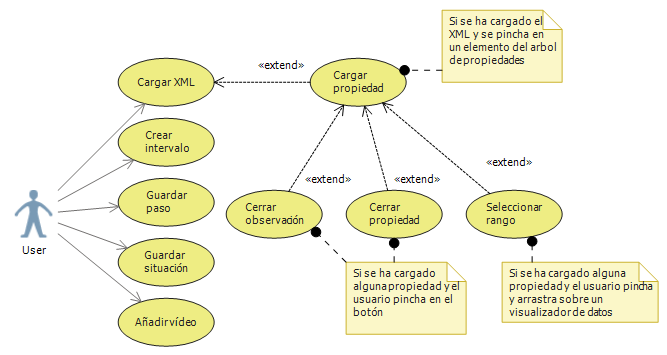
\includegraphics[width=1.0\linewidth]{./Figures/useCaseDiagram.png}
\caption[Diagrama de casos de uso]{Diagrama de casos de uso}
\label{fig:useCaseDiagram}
\end{figure}

\subsection{Casos de uso extendidos}
En esta secci\'on se proceder\'a a explicar brevemente cada caso de uso. %, dar una descripci\'on
%de que se hace, que actores toman parte, precondiciones, requisitos no funcionales, el flujo de
%eventos, as\'i como sus poscondiciones e interfaz gr\'afica asociada.

\subsubsection{Cargar XML}

\begin{table}[H]
	\begin{center}
		\rowcolors{2}{lightgray}{} %\rowcolors{<starting row index>}{<odd row color>}{<even row color>}
		\begin{tabular}{|l*{1}{p{10cm}}|}
			
			\multicolumn{2}{c}{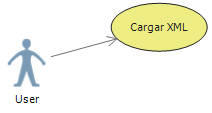
\includegraphics[width=0.36\linewidth]{./Figures/CargarXML.png}} \\
			\hline
		    Nombre                     & Cargar XML \\
		    Descripci\'on              & Carga un XML que contiene las propiedades
		    							 y las observaciones en el sistema. \'Unicamente
		    							 se cargan si el archivo valida contra el XSD.  \\ 
		    Actores                    & User  \\
		    Precondiciones             & Ninguna  \\
		    Requisitos no funcionales  & Ninguno  \\
		    Flujo de eventos           & \begin{enumerate}
		    								\item El usuario pincha en File -> Load XML.
		    								\item Se abre una ventana de selecci\'on de archivos.
		    								\item \textbf{Si el usuario quiere cargar un fichero}
		    								\begin{enumerate}
		    									\item Lo busca en el sistema de archivos [\ref{fig:AbrirXML1}]
		    									\item Lo selecciona y pincha en Abrir.
		    									\item \textbf{Si es un documento v\'alido}
		    									\begin{enumerate}
		    										\item Las observaciones y sus propiedades 
		    											  aparecen en el \'arbol lateral.
		    											  [\ref{fig:AbrirXML2}]
		    									\end{enumerate}
		    									\item \textbf{Si no}
		    									\begin{enumerate}
		    										\item Se muestra un error.
		    										[\ref{fig:AbrirXML3}]
		    									\end{enumerate}
		    								\end{enumerate}
		    								\item \textbf{Si no desea cargarlo}
		    								\begin{enumerate}
		    									\item Pincha en cancelar y se muestra un mensaje de que debe cargar un XML [\ref{fig:AbrirXML4}].
		    								\end{enumerate}
		    							 \end{enumerate} \\
		    Poscondiciones			   & El \'arbol contendr\'a las observaciones y 
		    							 propiedades si era un documento v\'alido, mostrar\'a
		    							 un error si era un documento inv\'alido, o mostrar\'a un aviso
                                         indicando de que se necesita cargar un XML para poder trabajar.  \\
		    Interfaz gr\'afica		   & Figuras \ref{fig:AbrirXML1}, \ref{fig:AbrirXML2},
		    							 \ref{fig:AbrirXML3} y \ref{fig:AbrirXML4}\\
		    \hline
		\end{tabular}
	\caption[Cargar XML]{Cargar XML}
	\label{Cargar XML}
	\end{center}
\end{table}

\subsubsection{A\~nadir v\'ideo}

\begin{table}[H]
	\begin{center}
		\rowcolors{2}{lightgray}{} %\rowcolors{<starting row index>}{<odd row color>}{<even row color>}
		\begin{tabular}{|l*{1}{p{10cm}}|}
			
			\multicolumn{2}{c}{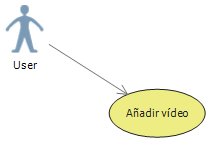
\includegraphics[width=0.4\linewidth]{./Figures/AnadirVideo.png}} \\
			\hline
		    Nombre                     & A\~nadir v\'ideo \\
		    Descripci\'on              & Abre un v\'ideo y lo a\~nade al contenedor
		    							 de v\'ideos si ya hab\'ia v\'ideos previamente
		    							 cargados. Si no, a\~nade tambi\'en un contenedor
		    							 de v\'ideos.  \\ 
		    Actores                    & User  \\
		    Precondiciones             & Ninguna  \\
		    Requisitos no funcionales  & Ninguno  \\
		    Flujo de eventos           & \begin{enumerate}
		    								\item El usuario pincha en Add Video.
		    								[\ref{fig:CargarVideo}]
		    								\item \textbf{Si el contenedor no de v\'ideos estaba
		    										      cargado}
	    									\begin{enumerate}
	    										\item Se crea y a\~nade un contenedor de v\'ideos.
	    									\end{enumerate}
	    									\item Se abre una ventana de selecci\'on de archivos.
		    								\item \textbf{Si el usuario quiere cargar v\'ideos}
		    								\begin{enumerate}
		    									\item Los busca en el sistema de archivos
		    									\item Los selecciona y pincha en Abrir.
		    									\item Se cargan si no estaban previamente cargados.
		    								\end{enumerate}
		    								\item \textbf{Si no desea cargarlo}
		    								\begin{enumerate}
		    									\item Pincha en cancelar.
		    								\end{enumerate}
		    							 \end{enumerate} \\
		    Poscondiciones			   & El contenedor con los nuevos v\'ideos a\~nadidos  \\
		    Interfaz gr\'afica		   & Figuras \ref{fig:CargarVideo}\\
		    \hline 
		\end{tabular}
	\caption[A\~nadir v\'ideo]{A\~nadir v\'ideo}
	\label{Anadir video}
	\end{center}
\end{table}
\pagebreak

\subsubsection{Cargar propiedad}

\begin{table}[H]
	\begin{center}
		\rowcolors{2}{lightgray}{} %\rowcolors{<starting row index>}{<odd row color>}{<even row color>}
		\begin{tabular}{|l*{1}{p{10cm}}|}
			
			\multicolumn{2}{c}{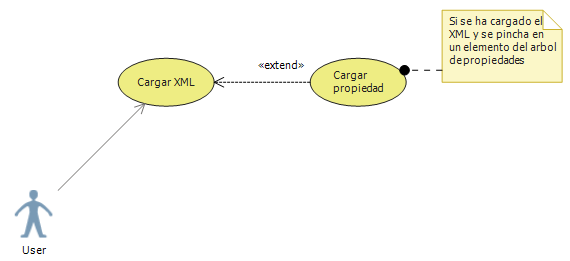
\includegraphics[width=0.6\linewidth]{./Figures/CargarPropiedad.png}} \\
			\hline
		    Nombre                     & Cargar propiedad \\
		    Descripci\'on              & Carga una propiedad en el contenedor de gr\'aficos
		    							 correspondiente a la observaci\'on a la que pertenece.
		    							 Tambi\'en puede a\~nadir propiedades en grupo, haciendo
		    							 doble click sobre el nombre de la observaci\'on. Si
		    							 el contenedor no est\'a creado, lo crea.  \\ 
		    Actores                    & User.  \\
		    Precondiciones             & Ninguna.  \\
		    Requisitos no funcionales  & Ninguno.  \\
		    Flujo de eventos           & \begin{enumerate}
		    								\item El usuario hace doble click en alg\'un elemento
		    									  del \'arbol de observaciones y propiedades.
		    								\item \textbf{Si el elemento es una observaci\'on}
		    								\begin{enumerate}
		    									\item Carga el contenedor si no estaba creado
		    									\item A\~nade todos sus hijos no cargados al
		    										  contenedor.
		    								\end{enumerate}
		    								\item \textbf{Si el elemento es una propiedad}
		    								\begin{enumerate}
			    								\item Crea el contenedor de la observaci\'on
			    									  a la que pertenece la propiedad seleccionada
			    									  si no estaba cargado.
			    								\item A\~nade la propiedad si no estaba cargada
			    									  previamente.
			    									  
		    								\end{enumerate}
		    							 \end{enumerate} \\
		    Poscondiciones			   & El contenedor de la observaci\'on y todas las 
		    							 propiedades de la observaci\'on o la propiedad
		    							 seleccionada dependiendo de d\'onde se haya hecho 
		    							 doble click y sincronizada con el rango existente, si es que lo hay. \\
		    Interfaz gr\'afica		   & Figuras \ref{fig:CargarObservacionPropiedad}\\
		    \hline
		\end{tabular}
	\caption[Cargar propiedad]{Cargar propiedad}
	\label{Cargar propiedad}
	\end{center}
\end{table}
\pagebreak

\subsubsection{Seleccionar rango}

\begin{table}[H]
	\begin{center}
		\rowcolors{2}{lightgray}{} %\rowcolors{<starting row index>}{<odd row color>}{<even row color>}
		\begin{tabular}{|l*{1}{p{10cm}}|}
			
			\multicolumn{2}{c}{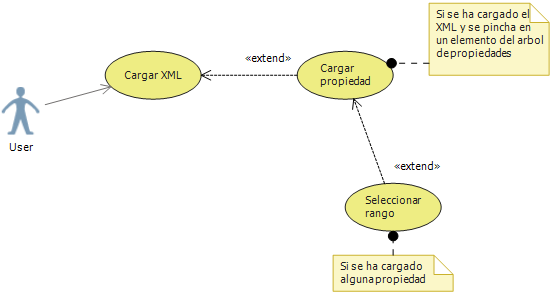
\includegraphics[width=1.0\linewidth]{./Figures/SeleccionarRango.png}} \\
			\hline
		    Nombre                     & Seleccionar rango \\
		    Descripci\'on              & Al pinchar y mover el rat\'on sobre un visualizador de datos,
		    							 se seleccionar\'a un rango en todos los visualizadores de datos
		    							 cargados en el sistema. \\ 
		    Actores                    & User  \\
		    Precondiciones             & Alguna propiedad tiene que estar cargada.  \\
		    Requisitos no funcionales  & Ninguno  \\
		    Flujo de eventos           & \begin{enumerate}
		    								\item El usuario pincha en un visualizador de datos.
		    								\item El usuario arrastra (manteniendo pinchado) el rat\'on.
		    								\begin{enumerate}
		    									\item Cada vez que el rango seleccionado cambia, se notifica al contenedor padre.
		    									\item El contenedor, notifica al repositorio de contenedores, para que todos
		    									se sincronicen con el dato proporciado.
		    									\item Se recorren todos los visualizadores de datos para sincronizarse con el nuevo
		    									valor.
		    								\end{enumerate}
		    								\item El usuario deja de pinchar, y se queda el rango seleccionado.
		    							 \end{enumerate} \\
		    Poscondiciones			   & El rango quedar\'a seleccionado en todos los 
		    							 visualizadores de datos
		    							 cargados en el sistema.  \\
		    Interfaz gr\'afica		   & Figuras \ref{fig:SeleccionarRango}\\
		    \hline
		\end{tabular}
	\caption[Seleccionar rango]{Seleccionar rango}
	\label{SeleccionarRango}
	\end{center}
\end{table}
\pagebreak

\subsubsection{Cerrar observaci\'on}
\begin{table}[H]
	\begin{center}
		\rowcolors{2}{lightgray}{} %\rowcolors{<starting row index>}{<odd row color>}{<even row color>}
		\begin{tabular}{|l*{1}{p{10cm}}|}
			
			\multicolumn{2}{c}{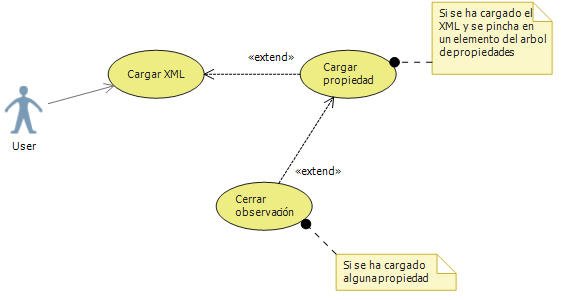
\includegraphics[width=1.0\linewidth]{./Figures/CerrarObservacion.png}} \\
			\hline
		    Nombre                     & Cerrar observaci\'on \\
		    Descripci\'on              & Elimina, tanto de manera visual, como de memoria, la observaci\'on
		    							 seleccionada y todos sus visualizadores de datos (propiedades) asociadas.  \\ 
		    Actores                    & User.  \\
		    Precondiciones             & La observaci\'on ten\'ia que estar cargada. \\
		    Requisitos no funcionales  & Ninguno.  \\
		    Flujo de eventos           & \begin{enumerate}
		    								\item El usuario pincha sobre la ``X" \ en la esquina
		    									  superior derecha de la observaci\'on.
		    								\item Se borra del repositorio, liberando sus recursos, y con ello,
		    									  sus propiedades.
		    								\item Finalmente se borra de la pantalla.
		    							 \end{enumerate} \\
		    Poscondiciones			   & El espacio de trabajo contendr\'a todas las observaciones
		    							 y propiedades menos la que se ha cerrado.  \\
		    Interfaz gr\'afica		   & Ninguna relevante.\\
		    \hline
		\end{tabular}
	\caption[Cerrar observaci\'on]{Cerrar observaci\'on}
	\label{Cerrar observacion}
	\end{center}
\end{table}
\pagebreak

\subsubsection{Cerrar propiedad}
\begin{table}[H]
	\begin{center}
		\rowcolors{2}{lightgray}{} %\rowcolors{<starting row index>}{<odd row color>}{<even row color>}
		\begin{tabular}{|l*{1}{p{10cm}}|}
			
			\multicolumn{2}{c}{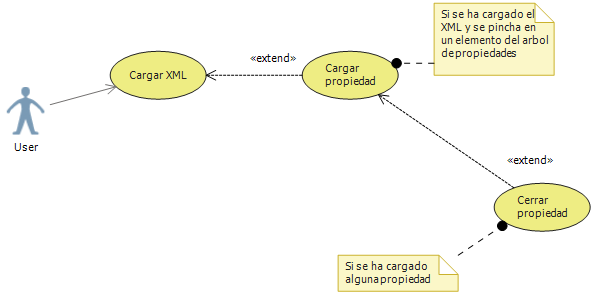
\includegraphics[width=1.0\linewidth]{./Figures/CerrarPropiedad.png}} \\
			\hline
			Nombre                     & Cerrar propiedad \\
			Descripci\'on              & Elimina, tanto de manera visual, como de memoria, la propiedad
									  	 seleccionada.  \\ 
			Actores                    & User.  \\
			Precondiciones             & La propiedad ten\'ia que estar cargada. \\
			Requisitos no funcionales  & Ninguno.  \\
			Flujo de eventos           & \begin{enumerate}
										 	\item El usuario pincha sobre la ``X" \ en la esquina
												  superior derecha de la propiedad.
											\item Se borra del contenedor al que estaba asociada.
											\item Finalmente se borra de la pantalla.
										 \end{enumerate} \\
			Poscondiciones			   & El espacio de trabajo contendr\'a todas las observaciones
										 y propiedades menos la propiedad que se ha cerrado.  \\
			Interfaz gr\'afica		   & Ninguna relevante\\
			\hline
		\end{tabular}
	\caption[Cerrar propiedad]{Cerrar propiedad}
	\label{Cerrar propiedad}
	\end{center}
\end{table}
\pagebreak

\subsubsection{Crear intervalo}
\begin{table}[H]
	\begin{center}
		\rowcolors{2}{lightgray}{} %\rowcolors{<starting row index>}{<odd row color>}{<even row color>}
		\begin{tabular}{|l*{1}{p{10cm}}|}
			
			\multicolumn{2}{c}{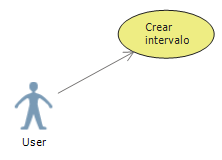
\includegraphics[width=0.4\linewidth]{./Figures/CrearIntervalo.png}} \\
			\hline
		    Nombre                     & Crear intervalo \\
		    Descripci\'on              & A\~nade el intervalo seleccionado
		    							 a los intervalos a guardar en el xml si
		    							 no se superpone con los que ya est\'an guardados.\\ 
		    Actores                    & User  \\
		    Precondiciones             & Alguna propiedad debe estar seleccionada
		    							 y un rango debe estar seleccionado.  \\
		    Requisitos no funcionales  & Ninguno  \\
		    Flujo de eventos           & \begin{enumerate}
		    								\item El usuario pincha Create interval.
		    								\item \textbf{Si el intervalo actual
		    								no se superpone con ninguno
		    								guardado previamente}
		    								\begin{enumerate}
		    									\item Se guarda el intervalo en la lista
		    									de intervalos a exportar.
		    									\item Se muestra un dialogo notificando que
		    									la operaci\'on se ha realizado correctamente. [\ref{fig:CrearIntervalo}]
		    								\end{enumerate}
		    								\item \textbf{Si se superpone}
		    								\begin{enumerate}
			    								\item Se muestra un dialogo notificando que
		    									el rango seleccionado se superpone con alguno
		    									guardado. [\ref{fig:CrearIntervaloError}]
		    								\end{enumerate}
		    								
		    							 \end{enumerate} \\
		    Poscondiciones			   & Se guardar\'a el nuevo intervalo en
		    							 lista de intervalos a exportar.  \\
		    Interfaz gr\'afica		   & Figuras \ref{fig:CrearIntervalo} y 
		    							 \ref{fig:CrearIntervaloError}\\
		    \hline
		\end{tabular}
	\caption[Crear intervalo]{Crear intervalo}
	\label{Crear Intervalo}
	\end{center}
\end{table}
\pagebreak

\subsubsection{Guardar paso}
\begin{table}[H]
	\begin{center}
		\rowcolors{2}{lightgray}{} %\rowcolors{<starting row index>}{<odd row color>}{<even row color>}
		\begin{tabular}{|l*{1}{p{10cm}}|}
			
			\multicolumn{2}{c}{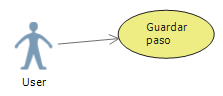
\includegraphics[width=0.4\linewidth]{./Figures/GuardarPaso.png}} \\
			\hline
		    Nombre                     & Guardar Paso. \\
		    Descripci\'on              & Guarda todos los intervalos creados
		    							 a disco con un elemento ra\'iz ``step".\\ 
		    Actores                    & User  \\
		    Precondiciones             & Ninguna.  \\
		    Requisitos no funcionales  & Ninguno  \\
		    Flujo de eventos           & \begin{enumerate}
		    								\item El usuario pincha en Save selected range -> Step. [\ref{fig:GuardarPaso1}]
		    								\item Se muestra un di\'alogo de guardado de datos.
		    								\item \textbf{Si el usuario decide guardar
		    								el fichero.}
		    								\begin{enumerate}
		    									\item Elige un nombre de fichero y pincha
		    									en guardar. [\ref{fig:GuardarPaso2}]
		    									\item El fichero se guarda en la carpeta
		    									especificada.
		    									\item Se borran todos los intervalos
		    									guardados.
		    								\end{enumerate}
		    								\item \textbf{Si pincha en cancelar}
		    								\begin{enumerate}
		    									\item Se cierra la ventana y no se borran
		    									los intervalos, para poder seguir trabajando.
		    								\end{enumerate}
		    								
		    							 \end{enumerate} \\
		    Poscondiciones			   & El fichero guardado en disco, o no,
		    						     dependiendo de las acciones del usuario.  \\
		    Interfaz gr\'afica		   & Figuras \ref{fig:GuardarPaso1} y \ref{fig:GuardarPaso2}\\
		    \hline
		\end{tabular}
	\caption[Guardar paso]{Guardar paso}
	\label{Guardar paso}
	\end{center}
\end{table}
\pagebreak

\subsubsection{Guardar situaci\'on}
\begin{table}[H]
	\begin{center}
		\rowcolors{2}{lightgray}{} %\rowcolors{<starting row index>}{<odd row color>}{<even row color>}
		\begin{tabular}{|l*{1}{p{10cm}}|}
			
			\multicolumn{2}{c}{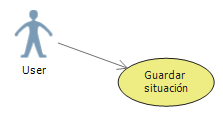
\includegraphics[width=0.4\linewidth]{./Figures/GuardarSituacion.png}} \\
			\hline
		    Nombre                     & Guardar situaci\'on \\
		    Descripci\'on              & Guarda todos los intervalos creados
  		    							 a disco con un elemento ra\'iz ``situation".\\ 
		    Actores                    & User  \\
		    Precondiciones             & Ninguna.  \\
		    Requisitos no funcionales  & Ninguno  \\
		    Flujo de eventos           & \begin{enumerate}
		    								\item El usuario pincha Save selected range -> 
		    								Situation. [\ref{fig:GuardarSituacion1}]
		    								\item Se muestra un di\'alogo de guardado de datos.
		    								\item \textbf{Si el usuario decide guardar
		    								el fichero.}
		    								\begin{enumerate}
		    									\item Elige un nombre de fichero y pincha
		    									en guardar. [\ref{fig:GuardarSituacion2}]
		    									\item El fichero se guarda en la carpeta
		    									especificada.
		    									\item Se borran todos los intervalos
		    									guardados.
		    								\end{enumerate}
		    								\item \textbf{Si pincha en cancelar}
		    								\begin{enumerate}
		    									\item Se cierra la ventana y no se borran
		    									los intervalos, para poder seguir trabajando.
		    								\end{enumerate}
		    								
										\end{enumerate} \\
			Poscondiciones			   & El fichero guardado en disco, o no,
										 dependiendo de las acciones del usuario.  \\
		    Interfaz gr\'afica		   & Figuras \ref{fig:GuardarSituacion1} y 
		    							 \ref{fig:GuardarSituacion2}\\
		    \hline
		\end{tabular}
	\caption[Guardar situaci\'on]{Guardar situaci\'on}
	\label{Guardar situacion}
	\end{center}
\end{table}
\pagebreak

\subsection{Figuras de los casos de uso}
\begin{figure}[H]
\centering
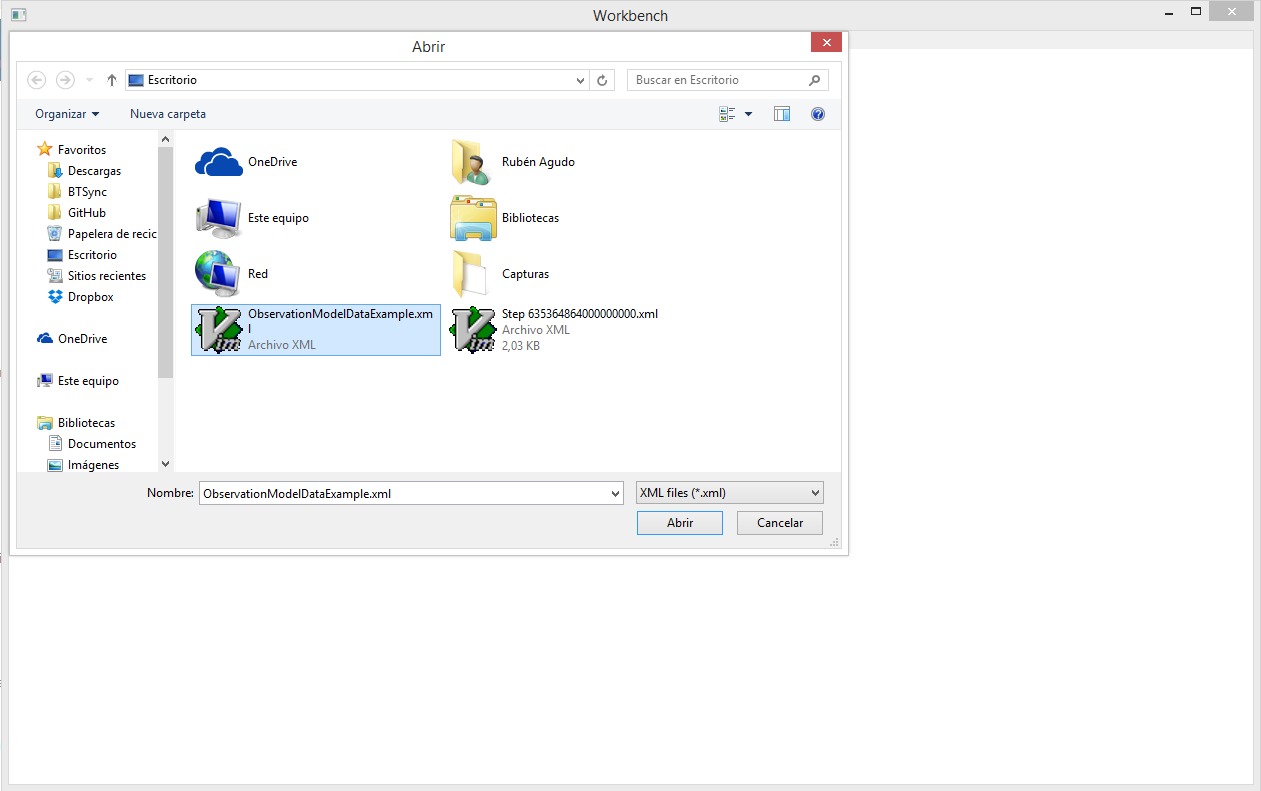
\includegraphics[width=1.0\linewidth]{./Figures/Capturas/AbrirXML1.PNG}
\caption{Abrir XML 1}
\label{fig:AbrirXML1}
\end{figure}

\begin{figure}[H]
\centering
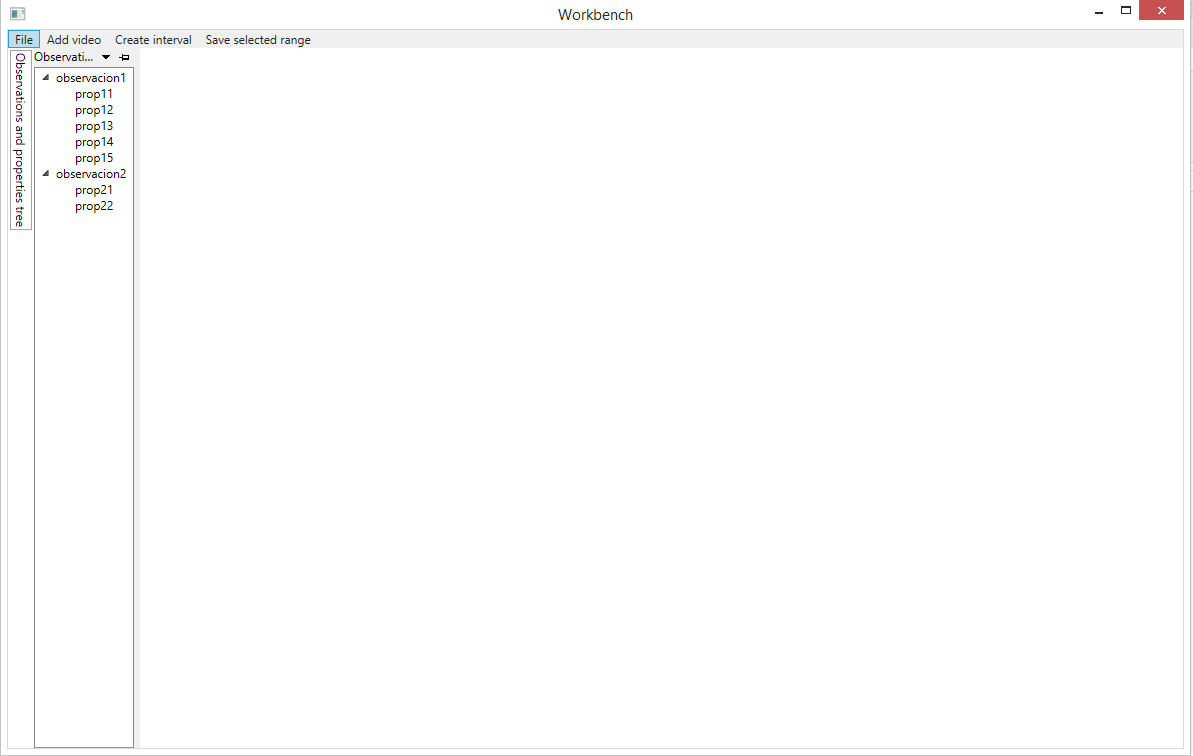
\includegraphics[width=0.9\linewidth]{./Figures/Capturas/AbrirXML2.PNG}
\caption{Abrir XML 2}
\label{fig:AbrirXML2}
\end{figure}

\begin{figure}[H]
\centering
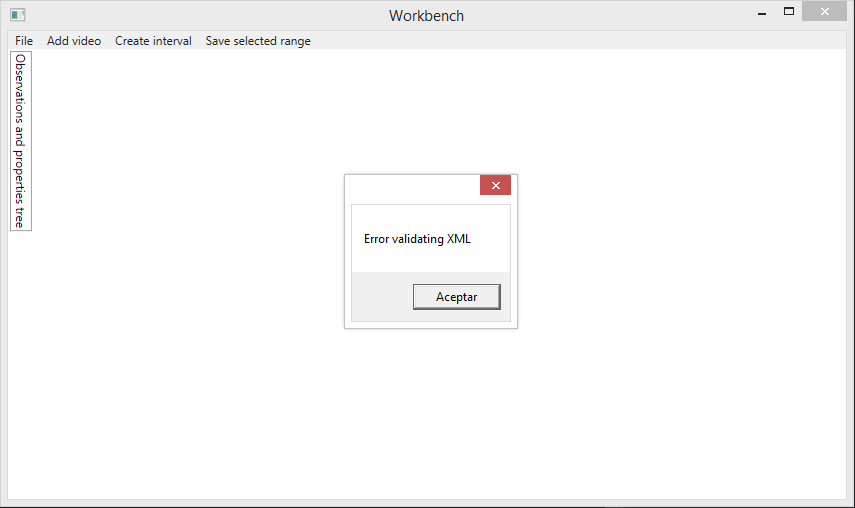
\includegraphics[width=0.9\linewidth]{./Figures/Capturas/AbrirXML3.PNG}
\caption{Abrir XML 3}
\label{fig:AbrirXML3}
\end{figure}

\begin{figure}[H]
\centering
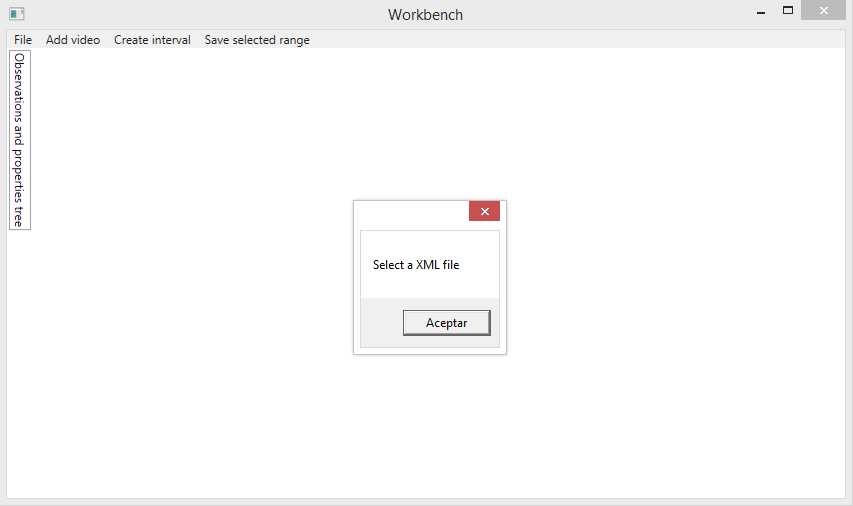
\includegraphics[width=0.9\linewidth]{./Figures/Capturas/AbrirXML4.PNG}
\caption{Abrir XML 4}
\label{fig:AbrirXML4}
\end{figure}

\begin{figure}[H]
\centering
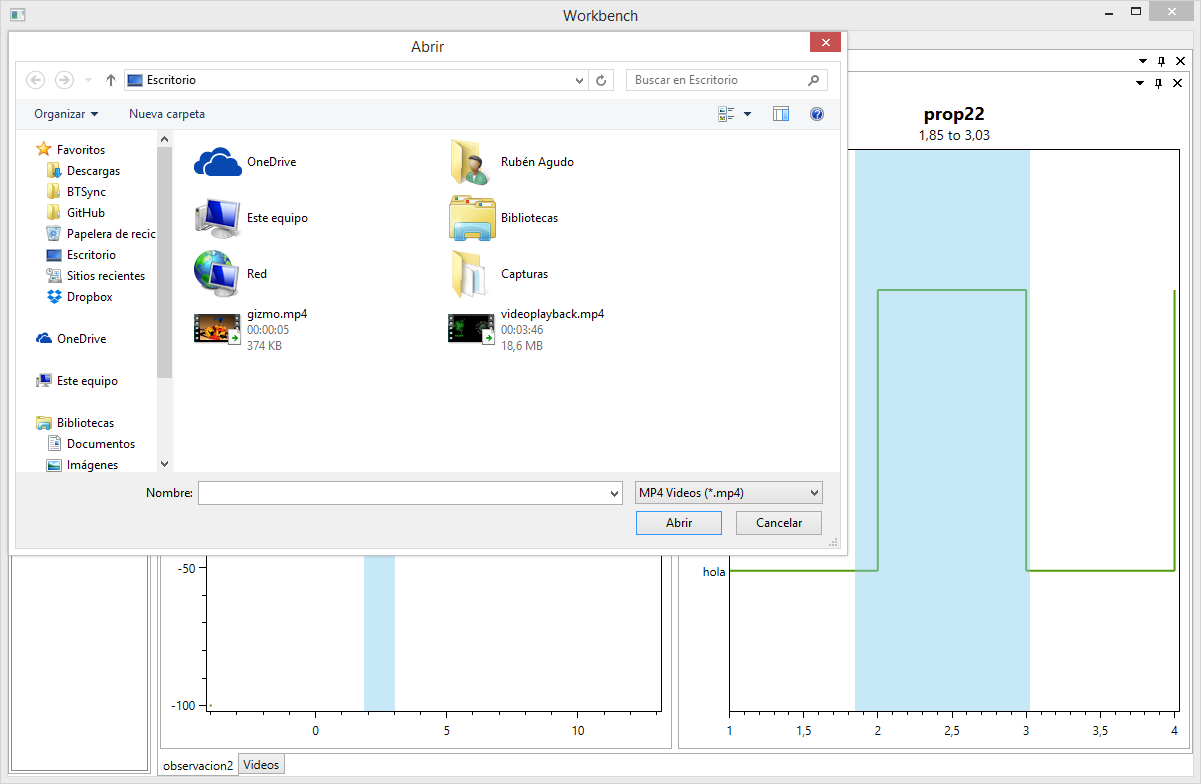
\includegraphics[width=0.9\linewidth]{./Figures/Capturas/CargarVideo.PNG}
\caption{Cargar V\'ideo}
\label{fig:CargarVideo}
\end{figure}

\begin{figure}[H]
\centering
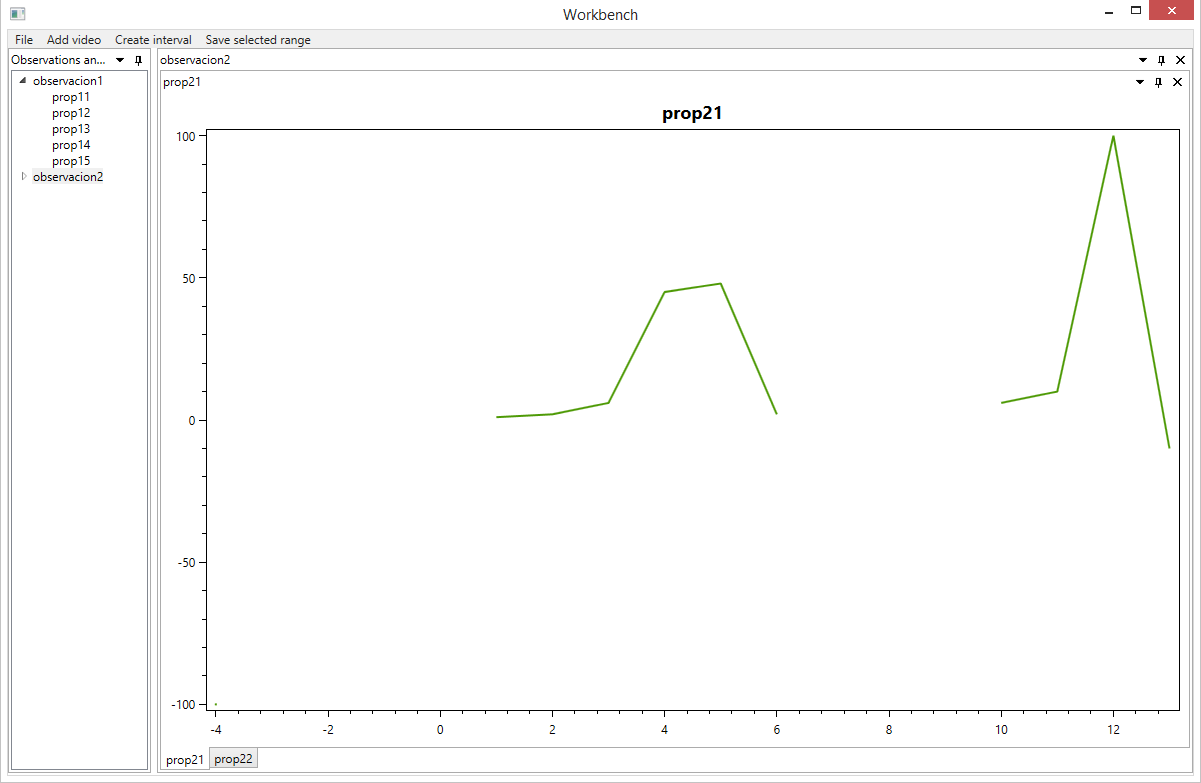
\includegraphics[width=0.9\linewidth]{./Figures/Capturas/CargarObservacionPropiedad.PNG}
\caption{Cargar Observaci\'on o Propiedad}
\label{fig:CargarObservacionPropiedad}
\end{figure}

\begin{figure}[H]
\centering
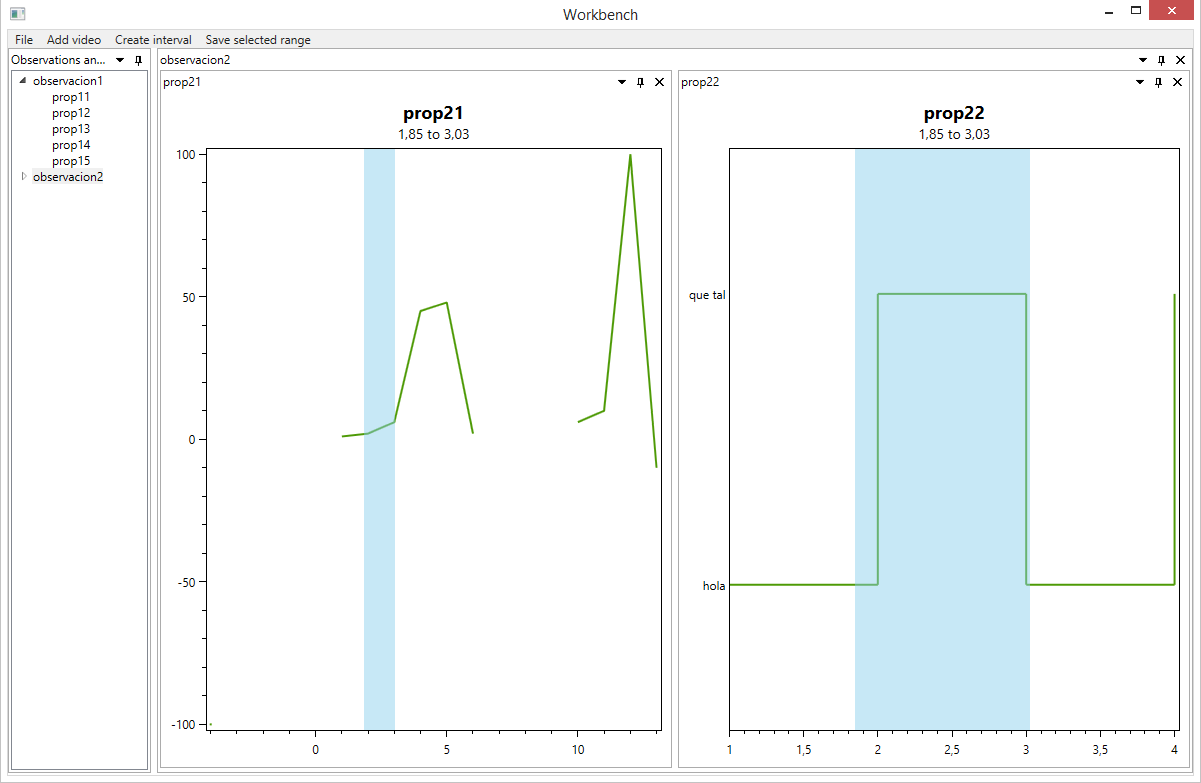
\includegraphics[width=0.9\linewidth]{./Figures/Capturas/SeleccionRango.PNG}
\caption{Seleccionar rango}
\label{fig:SeleccionarRango}
\end{figure}

\begin{figure}[H]
\centering
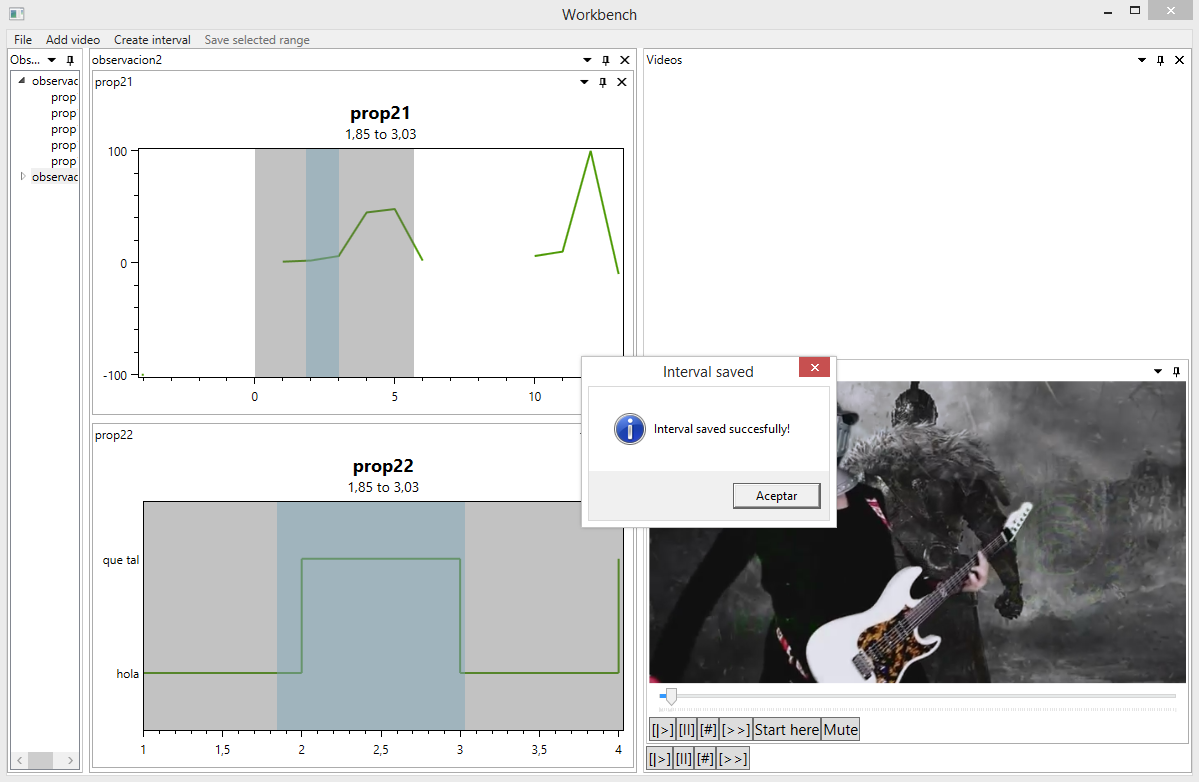
\includegraphics[width=0.9\linewidth]{./Figures/Capturas/IntervaloCreado.PNG}
\caption{Crear intervalo}
\label{fig:CrearIntervalo}
\end{figure}

\begin{figure}[H]
\centering
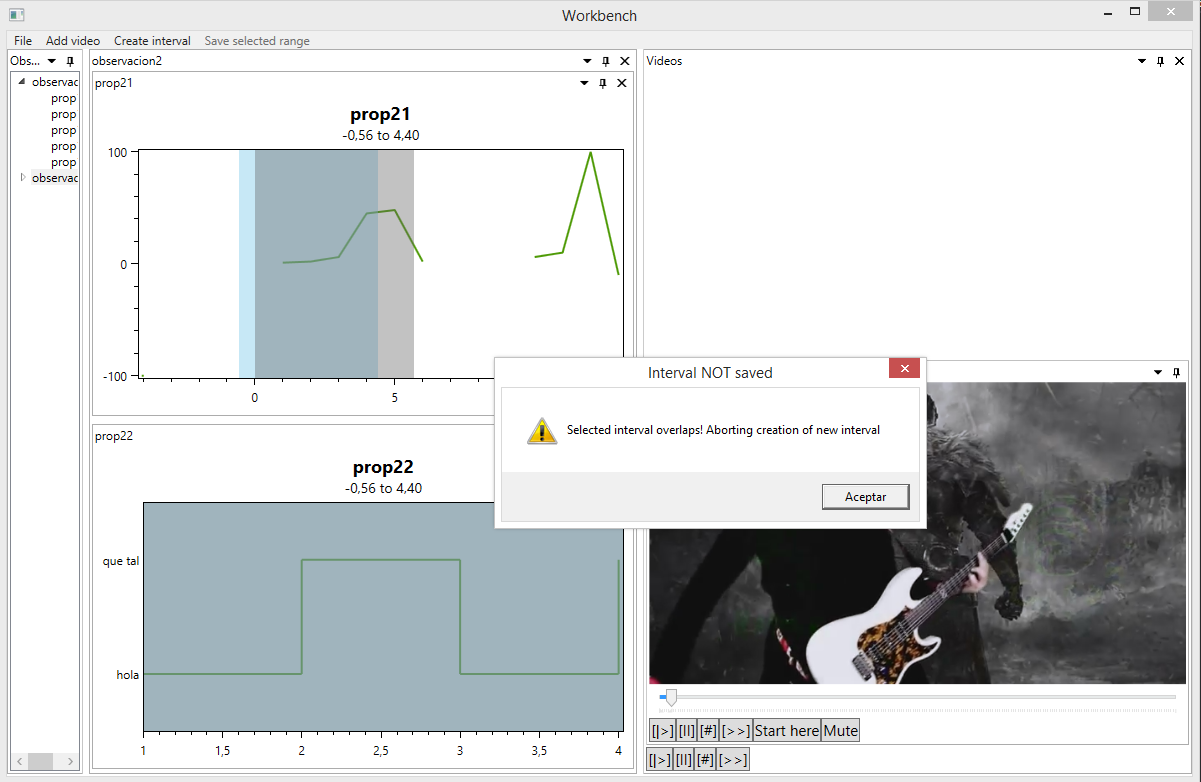
\includegraphics[width=0.9\linewidth]{./Figures/Capturas/IntervaloCreadoError.PNG}
\caption{Crear intervalo con  error}
\label{fig:CrearIntervaloError}
\end{figure}

\begin{figure}[H]
\centering
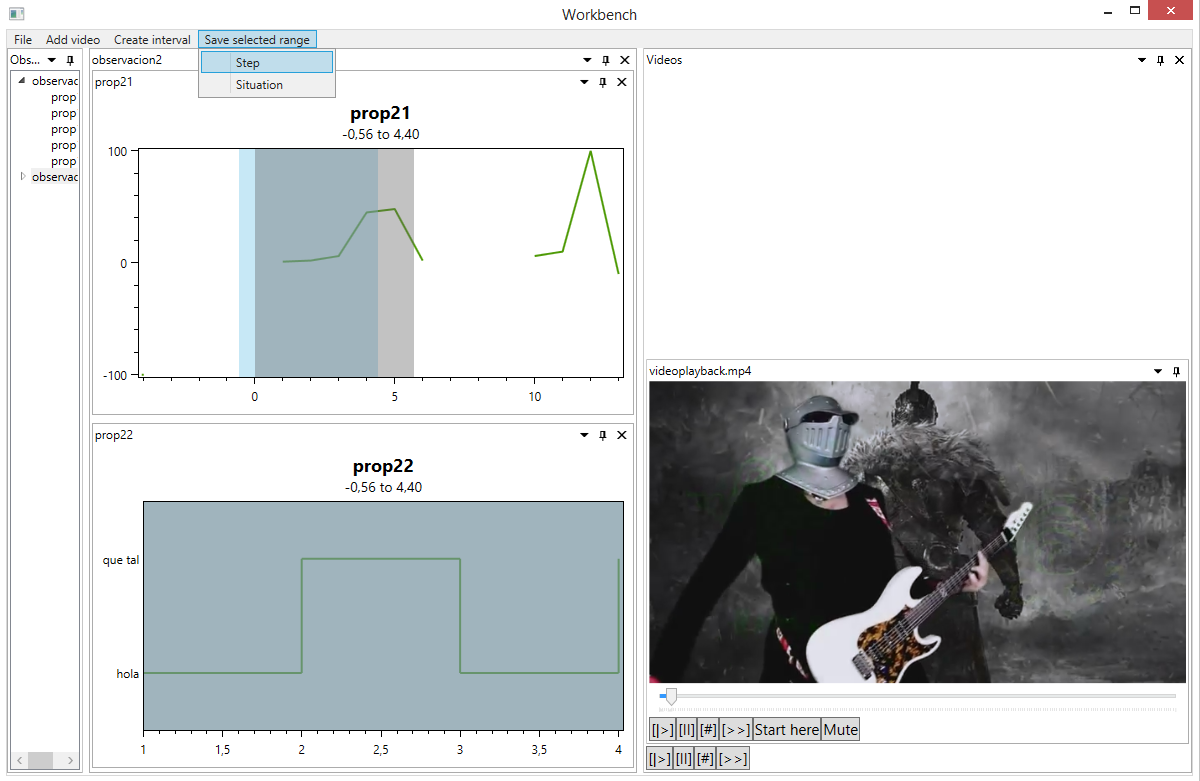
\includegraphics[width=0.9\linewidth]{./Figures/Capturas/GuardarPaso1.png}
\caption{Guardar paso 1}
\label{fig:GuardarPaso1}
\end{figure}

\begin{figure}[H]
\centering
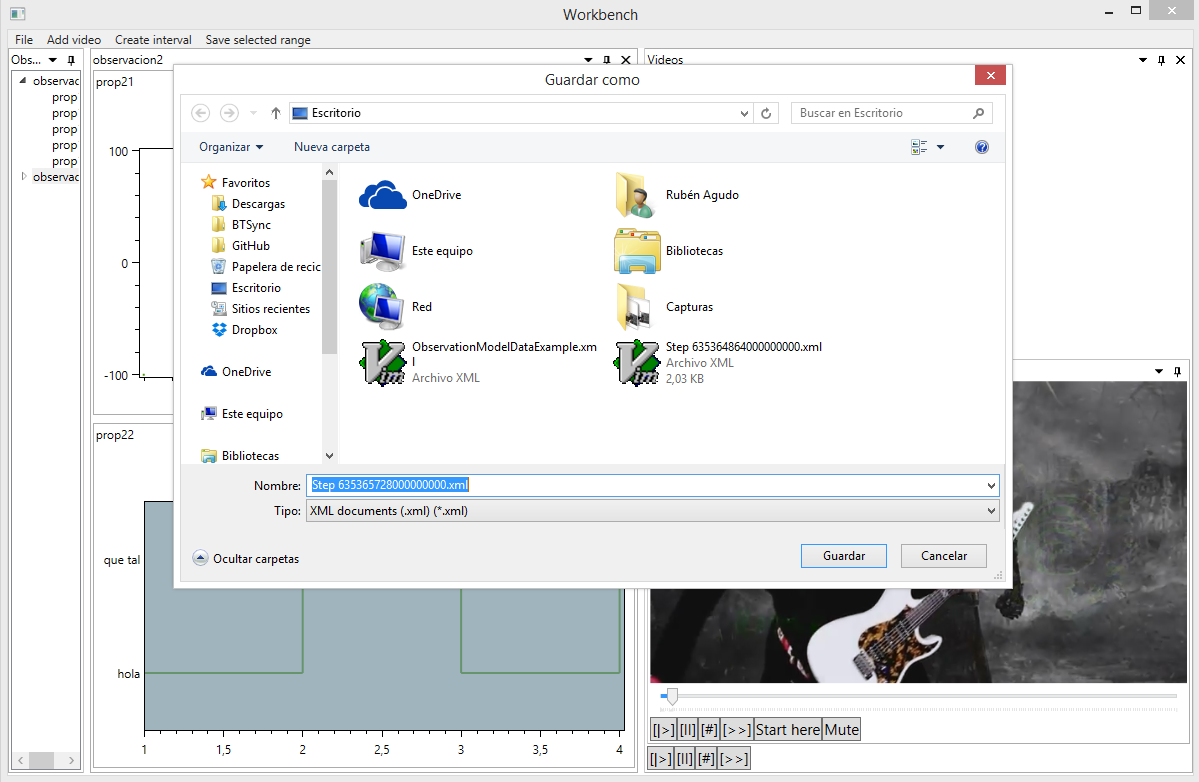
\includegraphics[width=0.9\linewidth]{./Figures/Capturas/GuardarPaso2.PNG}
\caption{Guardar paso 2}
\label{fig:GuardarPaso2}
\end{figure}

\begin{figure}[H]
\centering
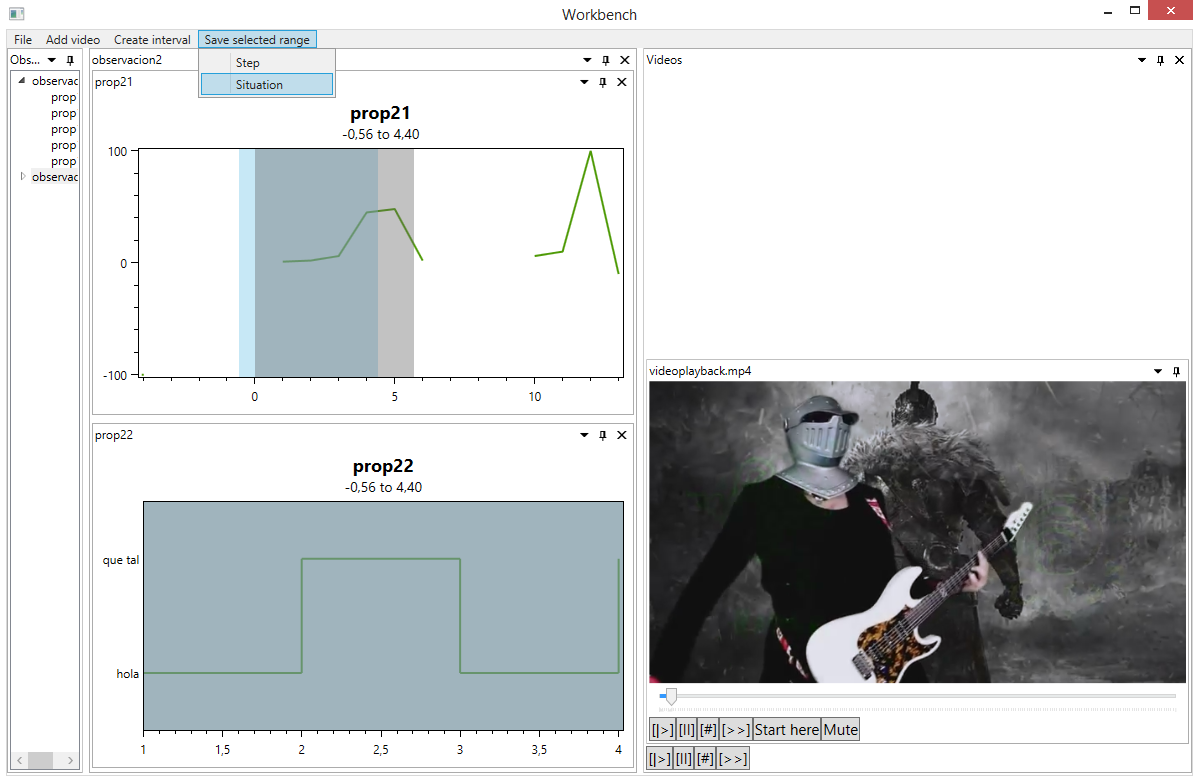
\includegraphics[width=0.9\linewidth]{./Figures/Capturas/GuardarSituacion1.png}
\caption{Guardar situaci\'on 1}
\label{fig:GuardarSituacion1}
\end{figure}

\begin{figure}[H]
\centering
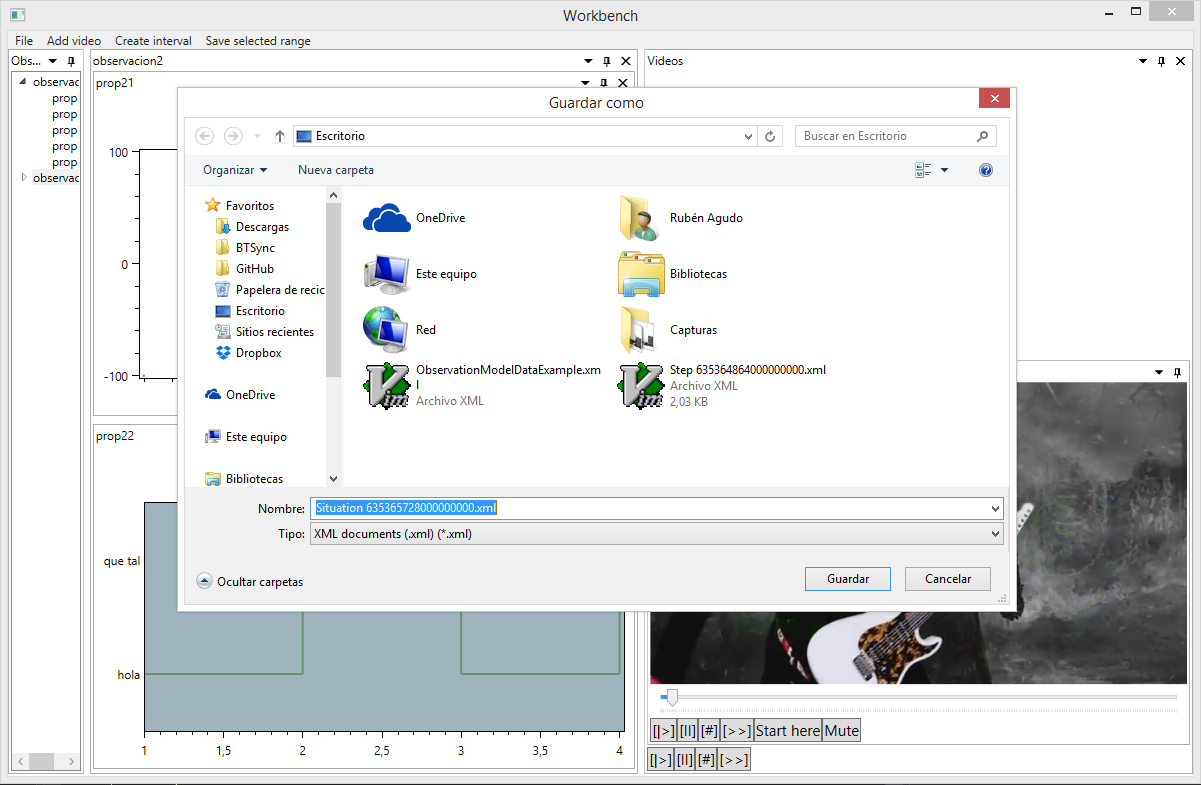
\includegraphics[width=0.9\linewidth]{./Figures/Capturas/GuardarSituacion2.PNG}
\caption{Guardar situaci\'on}
\label{fig:GuardarSituacion2}
\end{figure}


\section{Modelo de dominio}
Los datos que se guardan son ciertamente bastante simples, ya que para la tripleta Instante, Observaci\'on y Propiedad,
toma un \'unico valor posible. 

La Figura \ref{fig:ModelodeDominio} representa tanto los datos de entrada del software, tanto los datos
de salida.

\begin{figure}[H]
\centering
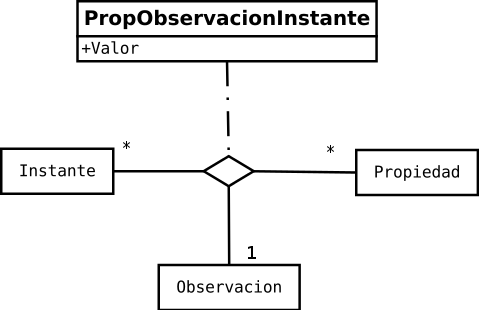
\includegraphics[width=0.7\linewidth]{./Figures/ModelodeDominio}
\caption[Modelo de dominio]{Modelo de dominio}
\label{fig:ModelodeDominio}
\end{figure}

   \chapter{An\'{a}lisis y dise\~{n}o}
%\newpage
%Cómo se plantea el desarrollo del trabajo. En que partes se 
%divide la solución, justificando dicha división y explicando 
%cada una de las partes.

%En aquellos trabajos donde sea aplicable se documentará 
%usando el modelo de dominio, el diagrama de clases, los 
%módulos/paquetes del software desarrollado, etc.

\section{An\'{a}lisis}
Los datos que ha de guarda el software estar\'an en un XML. El XML se divide en:
\begin{itemize}
	\item Observaciones
	\item Propiedades
	\item Instantes
\end{itemize}

Por tanto se ha decidido guardar la lista de Observaciones, cada observaci\'on contiene la lista de Propiedades 
y cada Propiedad una lista de Instantes en los que se guardar\'a los valores.

El rango seleccionado en cada propiedad estar\'a sincronizado con el resto de propiedades cargadas. 
Ya que no tiene sentido que por ejemplo, la observaci\'on ``coche", 
que tiene como propiedades ``velocidad" \ y ``aceleraci\'on" \ tengan distintos rangos 
seleccionados, ya que si en ``velocidad" \ seleccionamos [1, 3] y en ``aceleraci\'on" \ [2, 4], 
¿Qu\'e guardamos? ¿El primero o el segundo? Por tanto, ya que todas las propiedades suceden al
mismo tiempo se sabe que est\'an relacionadas, por lo que es necesario que los rangos est\'en
sincronizados.

A la hora de guardar, tampoco podr\'an guardarse distintos rangos que se solapen con los
previamente creados para un mismo paso o situaci\'on
. Ya que en un mismo instante de tiempo, no pueden estar sucediendo dos cosas al mismo tiempo.
Por ejemplo, un brazo no puede estar levant\'andose, y baj\'andose al mismo tiempo.

Gr\'aficamente las clases se dividen de dos maneras: Contenedores y clases ``hoja".
El programa puede verse como una estructura de \'arbol, en las que de la ventana principal,
cuelgan los contenedores de v\'ideo y gr\'aficos, y de los de gr\'aficos cuelga el 
visualizador de datos.

Los v\'ideos tienen la misma estructura. Tambi\'en disponen de un contenedor en el que se
guardan todos los v\'ideos. Esos v\'ideos, ir\'an sincronizados con los gr\'aficos, mostrando
el progreso, para que sea m\'as intuitivo seleccionar los rangos.

\section{Dise\~{n}o}
No se ha seguido un proceso de dise\~no cl\'asico, en el cual antes de empezar a programar se realiza
un dise\~no exhaustivo, en el que se modelan las clases, atributos, incluso algunos m\'etodos y
llamadas entre m\'etodos.

Se ha seguido un proceso iterativo de dise\~no. En cada sprint, se iba construyendo sobre lo anterior, y refactorizando
y mejorando lo que hab\'ia previamente. Ha sido un proceso en el que se ha sido muy cr\'itico con lo que ya estaba
hecho, en ning\'un momento se ha dejado algo porque ``funciona", siempre se ha intentado mejorar lo que ya hab\'ia.

En cada iteraci\'on se iba consolidando el trabajo previo. Y si se llegaba a una situaci\'on en la que hab\'ia que redise\~nar
partes grandes se hac\'ia sin miedo.

\subsection{Librer\'{i}as usadas}
\begin{itemize}
    \item \textbf{AvalonDock:} 
    Es una librer\'{i}a que permite crear ventanas acoplables en WPF, al m\'as puro estilo Eclipse o Visual Studio. Es
    c\'{o}digo abierto y gratuita, pese a que tambi\'{e}n dispone de una versi\'{o}n profesional que es de pago. La usada en este proyecto
    ha sido la versi\'{o}n gratuita o \emph{community}. La versi\'{o}n usada esta licenciada bajo licencia BSD.
    \item \textbf{OxyPlot:}
    Biblioteca de c\'odigo abierto para realizar gr\'aficos. Permite visualizar gr\'aficos cont\'inuos, discretos, 
    selecci\'on de rangos. Licenciada bajo los t\'erminos de la licencia MIT.
\end{itemize}

\subsection{Patrones utilizados}

\subsubsection{MVVM}
MVVM es un patr\'{o}n de dise\~{n}o creado por Microsoft. Intenta conseguir las ventajas de Model-View-Controller como adem\'as una separaci\'{o}n total
de la vista del controlador. De esta forma los dise\~{n}adores de UI pueden centrar todos sus esfuerzos en crear la interfaz sin preocuparse 
del c\'{o}digo de la aplicaci\'{o}n, ya que se asume que la interfaz va a cambiar mucho durante el ciclo de vida de la aplicaci\'{o}n. Pero,
¿Si separamos totalmente la vista del modelo, como se comunican? En MVC el encargado de eso es el controlador, pero un detalle importante es 
que el c\'{o}digo referente a la vista debe tener llamadas a funciones en el lenguaje utilizado.

Y en este punto es donde la parte VM \footnote{View-Model} toma sentido. el View-Model es una abstracci\'{o}n de la vista, y que es el objetivo 
de los enlaces de datos. El View-Model expone los datos del modelo para que el creador de interfaces pueda enlazar los elementos de la UI
con los datos del modelo (bien utilizando orientaci\'{o}n a objetos o exponiendo los datos de la BD) sin escribir una sola l\'{i}nea de 
c\'{o}digo .NET.

\paragraph{Elementos de MVVM}

\begin{itemize}
    \item \textbf{Model:} Dentro del patr\'{o}n MVC corresponde al modelo de dominio utilizando orientaci\'{o}n a objetos, o a los datos
    representados por una BD.
    \item \textbf{View:} La interfaz de usuario con sus botones, cajas de texto etc.
    \item \textbf{View Model:} Es la \emph{Vista del Modelo}, siendo una abstracci\'{o}n que sirve de mediadora y que expone los datos
    del modelo a la vista, para que esta \'{u}ltima pueda utilizarlas mediante enlaces de datos simples que no requieren de c\'{o}digo, sino
    que se crean mediante XAML. Realmente, no s\'{o}lo expone los datos, si no que adem\'as convierte los datos del modelo, en datos de vista, listos
    para ser visualizados.
\end{itemize}

\paragraph{Cr\'{i}ticas}
Es curioso que las principales cr\'{i}ticas provengan de su creador, Josh Gossman, el cual dice que utilizar a la fuerza MVVM para operaciones simples
de UI es una exageraci\'{o}n y que si los enlaces de datos si no se gestionan correctamente puede llevar a un consumo excesivo de 
memoria de la aplicaci\'{o}n \cite{MVVM:Criticism}

\paragraph{Uso en el TFG}
El patr\'on MVVM no se ha utilizado tal y como fue concebido. Pero si se ha mantenido la separaci\'on entre
las tres partes del software. Se han creado los ViewModels tal y como se recomienda en el patr\'on, pero no
se han podido utilizar los enlaces de datos, ya que para poder usarlos hay que establecer un contexto de datos,
y en este caso es din\'amico. Adem\'as se necesitan m\'as cosas que simplemente visualizar unos datos. Pero
pese a todo, el software se ha construido en torno a la idea del MVVM aunque no se haya podido aplicar exactamente
como se recomienda.

\subsubsection{Iterator}
Si bien el titulo alude al patr\'{o}n \emph{Iterator} .NET no dispone como Java de las interfaces \emph{Iterable} ni
\emph{Iterator}.
En cambio, dispone de las interfaces llamadas \emph{IEnumerator<T>} e \emph{IEnumerable<T>} 
que ofrecen una funcionalidad equivalente a las de Java.

Se ha decidido utilizar este patr\'{o}n por los siguientes motivos:
\begin{enumerate}
    \item \textbf{Abstracci\'{o}n:}
    Al utilizar este patr\'{o}n se pueden obtener los elementos de un contenedor, que puede ser un \emph{array}, una \emph{LinkedList<>}...
    cualquier clase que implemente la interfaz \emph{IEnumerable<T>} sin
    exponer su representaci\'{o}n interna, aumentando la seguridad y previniendo que una clase tenga acceso a cosas que no deba.
    
    \item \textbf{Facilidad de uso:}
    Siempre es preferible utilizar cosas que nos provea el \emph{framework}, ya que no es necesario perder el tiempo en banalidades como 
    recorrer una lista, y probablemente lo haremos menos eficientemente que lo actualmente programado. De todas formas, si necesitamos
    recorrerlo de una manera particular, y que sabemos hacerlo muy eficientemente, no hay problema en no seguir el patr\'{o}n, ya que no son
    normas, si no recomendaciones.
    
    \item \textbf{Prevenci\'{o}n de errores:}
    Relacionado con lo anterior. Si se pierde el tiempo a\~{n}adiendo l\'{i}neas extra la probabilidad de que se cometa un error 
    aumenta. Y aunque no haya sido probado emp\'{i}ricamente, se tiende a pensar que \emph{¿Como me voy a equivocar en 
    recorrer un array? ¡Pero si est\'{a} perfecto!}. 
    Y ello llevar\'{a} a malgastar m\'{a}s aun algo tan preciado como el tiempo. Pero al menos servir\'a para darse cuenta del error y 
    se ver\'a lo \'{u}tiles que son los patrones.
\end{enumerate}

\paragraph{Uso en el TFG}
Este patr\'on ha sido muy \'util en todo aquello que tenga que ver con recorrer datos. Por ejemplo a la hora de
sincronizar el rango seleccionado entre los visualizadores de datos. Adem\'as en C\# se realiza de una manera 
muy sem\'antica.

\begin{lstlisting}[language=C, numbers=left, showspaces=false, breaklines=true, tabsize=2]
	public partial class UC_ChartCOntainer : UserControl 
	{
		private SortedSet<UC_DataVisualizer> datavisualizers;
		
		internal void updateSelections(double[] selectedRange)
		{
			foreach(UC_DataVisualizer datav in datavisualizers) 
			{
				datav.updateRangeSelection(selectedRange);
			}
		}
	}
\end{lstlisting}

Como se puede ver en el trozo de c\'odigo, se ha podido iterar a trav\'es de todos los elementos
de \emph{datavisualizers} sin tener que comprobar si hay un elemento siguiente, el tama\~no del
elemento sobre el que se quiere iterar... Y adem\'as como se ha dicho antes, este
c\'odigo se ha vuelto mucho mas legible, ya que puede leerse de la 
siguiente manera: ``para cada datav en datavisualizers,
actualizar el rango seleccionado de datav con el rango obtenido por par\'ametro".
Concretamente, el ejemplo hace referencia al m\'etodo de sincronizaci\'on de rangos de las
observaciones. Lo que se ha hecho es recorrer todas las propiedades cargadas de una observaci\'on para
sincronizarlo con el rango dado como par\'ametro.

\subsubsection{Singleton}
Patr\'on de dise\~no b\'asico que consigue que una clase tenga una \'unica instancia durante toda la ejecuci\'on del software, siendo 
accesible por toda la aplicaci\'on.

En general, hay dos maneras de crear una clase Singleton.

\paragraph{Lazy} La inicializaci\'on \emph{Lazy} o \emph{perezosa} \'unicamente crea la instancia cuando la necesita, es decir, la primera vez.
Para conseguirlo, cada vez que se intenta obtener la instancia se comprueba si ya hab\'ia sido previamente instanciada. Uno de los problemas de
la inicializaci\'on perezosa es que en entornos multihilo da problemas si no se obtiene un bloqueo exclusivo de la clase.

Una inicializaci\'on perezosa con comprobaci\'on doble de bloqueo se realiza as\'i:
\begin{lstlisting}[language=C, numbers=left, showspaces=false, breaklines=true, tabsize=2]
    public class GraphicsActions 
    {
        private static object myLock = new object();
        private static GraphicActions myGraphicActions;
        
        public static GraphicActions getMyGraphicActions()
        {
            if (myGraphicActions == null)
            {
                lock (myLock)
                {
                    if (myGraphicActions == null)
                    {
                        myGraphicActions = new GraphicActions();
                    }
                }
            }
            
            return myGraphicActions;
        }
    }
\end{lstlisting}

En .NET 4.0 fue incluida la clase \emph{Lazy<T>} que realiza ese tipo de inicializaci\'on.

\paragraph{Eager} En la inicializaci\'on \emph{Eager} o \emph{ansiosa} se crea la nueva instancia siempre. En este m\'etodo no hay problemas
en entornos multihilo, pero tiene un mayor coste computacional si la constructora es muy compleja.

Una inicializaci\'on ansiosa se realiza de la siguiente manera:
\begin{lstlisting}[language=C, numbers=left, showspaces=false, breaklines=true, tabsize=2]
    public class GraphicsActions 
    {
        private static GraphicActions myGraphicActions = new GraphicActions();
        
        public static GraphicActions getMyGraphicActions()
        { 
            return myGraphicActions;
        }
    }
\end{lstlisting}

\paragraph{Cr\'iticas}Pese a haberse utilizado el patr\'on Singleton, muchos desarrolladores desaconsejan su uso, ya que implican
una violaci\'on del Principio de Responsabilidad \'Unica del que se hablar\'a m\'as adelante. Y lo viola porque
la clase Singleton tendr\'ia dos responsabilidades, controlar que s\'olo exista una \'unica instancia y adem\'as
toda su l\'ogica de negocio \cite{Singleton:EVIL}.

Por otro lado, tambi\'en tiene como inconveniente una de las m\'aximas de la programaci\'on: Las variables globales
son malas. Pues por si no fuera poco, un Singleton es una clase global \cite{Singleton:EVIL}.

\paragraph{Uso en el TFG}
Pese a las cr\'iticas del p\'arrafo anterior, se ha utilizado en aquellos elementos que s\'olo iban a tener
una instancia. Concretamente \emph{VideoActions}, \emph{GraphicActions} y \emph{XMLExport}. Al
hacerlos accesibles desde todo el c\'odigo, se ha facilitado mucho la tarea al desarrollador para utilizarlo.

\subsection{SOLID}
SOLID es un acr\'{o}nimo mnem\'{o}nico acu\~{n}ado a comienzos de la d\'{e}cada de los 2000 por 
Robert C. Martin \cite{SOLID:ADefinition}
que representa cinco principios b\'{a}sicos de la programaci\'{o}n orientada a objetos y del dise\~{n}o de software.

SOLID merece un apartado en esta memoria ya que se ha intentado cumplir en el mayor grado posible los cinco principios.

Los principios son los siguientes:
\subsubsection{Single responsibility principle}
Traducido al castellano: Principio de responsabilidad \'{u}nica. El nombre puede llevar a enga\~{n}o ya que Martin define como 
\emph{responsabilidad}
a una \emph{raz\'{o}n de cambio} \cite{SOLID:SRP} y concluye que una clase, debiera tener, una, y solamente una raz\'{o}n 
para cambiar.

Por ejemplo, imaginemos que disponemos de una clase, o m\'{o}dulo que compila e imprime un informe. 
Ese informe puede cambiar por dos razones, de estilo, o de contenido. 

El principio de responsabilidad \'{u}nica dice que una clase solo debiera cambiar por un motivo, y por 
tanto tendr\'{i}amos que separar el m\'{o}dulo en dos: El que compila el informe, y el que lo imprime.

Utilizando este principio volveremos nuestro c\'{o}digo m\'as robusto, ya que un cambio en una clase, no 
deber\'{i}a afectar a la salida, y por tanto los siguientes m\'{o}dulos que se alimenten de esa clase.

\paragraph{Uso en el TFG}
Si bien el principio de responsabilidad \'unica no es algo que se aplique de manera directa, es decir,
no es si sucede A entonces haz B. Pero hay en algunas situaciones en las que se cumple este principio.
Por ejemplo, en la clase \emph{UC\_ChartContainer} se manten\'ia un repositorio de Observaciones
y adem\'as de propiedades. Se ve, que esta clase tiene dos razones de cambio. Una es por las propiedades
(a\~nadir, borrar etc) como por las observaciones (a\~nadir, borrar etc). Al incumplirse el principio,
la clase ha de separarse en dos. En un repositorio de propiedades, y en un repositorio de observaciones.

En este caso concreto, no se separ\'o en dos clases, sino que la colecci\'on de propiedades, pas\'o a ser
responsabilidad de cada \emph{UC\_ChartContainer}.

\subsubsection{Open/Closed principle}
El principio abierto / cerrado \cite{SOLID:OCP} implica que una clase est\'{a} abierta a la extensi\'{o}n pero cerrada a la 
modificaci\'{o}n. Ya que un cambio en el
funcionamiento de una clase har\'{i}a que se tambalease la estabilidad de nuestro software.

\paragraph{Uso en el TFG}
Ciertamente este principio no se ha utilizado, ya que est\'a mas pensado para ser usado en
c\'odigo que ya est\'a en producci\'on, no mientras el software est\'a en desarrollo.

\subsubsection{Liskov's substitution principle}
El principio de sustituci\'{o}n de Liskov \cite{SOLID:LSP} \footnote{\url{http://pmg.csail.mit.edu/~liskov/}} 
sostiene que cualquier subtipo de una clase
debe poder sustituir a su supertipo sin que haya un cambio de comportamiento.

M\'{a}s formalmente: Si \textbf{S} es un subtipo de \textbf{T} entonces \textbf{T} puede sustituirse por \textbf{S} y 
conservar su exactitud, tarea que realiza etc.

\paragraph{Uso en el TFG}
Este principio se cumple claramente, ya que para incumplirlo habr\'ia que sobreescribir alg\'un m\'etodo de la superclase
y que funcionase diferente de como funciona en la superclase. 

T\'omese como ejemplo las clases \emph{XMLValidation} y \emph{XMLLoader}.
Si \emph{XMLValidation} no fuera abstracta, podr\'ia ser sustituida por \emph{XMLLoader}
sin alterar su funcionalidad base, ya que \emph{XMLLoader} no sobreescribe el m\'etodo de la clase base. Lo mismo
sucede con los ViewModels. Ambas clases derivadas podr\'ian sustituir a la clase abstracta sin cambiar su funcionalidad. Es
decir, aunque las clases derivadas hayan sustituido a la clase padre, las clases derivadas siguen teniendo la funcionalidad
de la clase base intacta.

\subsubsection{Interface segregation principle}
El principio de segregaci\'{o}n de interfaces dice que es mejor tener muchas interfaces espec\'{i}ficas, 
que una gran interfaz que contenga todo \cite{SOLID:ISP}.

De esta manera evitamos que haya partes del software que dependan de m\'{e}todos que no influyen en esa clase.

\paragraph{Uso en el TFG}
Al s\'olo tener una interfaz propia, y que adem\'as tiene un \'unico m\'etodo, se cumple siempre, ya que
cada vez que una clase implemente esa interfaz es porque se requiere ese m\'etodo, si no, no tendr\'ia sentido
implementarla.

\subsubsection{Dependency inversion principle}
El principio de Inversi\'{o}n de dependencia \cite{SOLID:DIP} dice que:
\begin{enumerate}
    \item Los m\'{o}dulos de alto nivel no deben depender en m\'{o}dulos de bajo nivel. Ambos deben depender de abstracciones
    \item Las abstracciones no deben depender en los detalles. Los detalles deben depender de las abstracciones.
\end{enumerate}

\paragraph{Uso en el TFG}
Este principio es el \'unico que no se cumple. Ya que los m\'odulos de alto nivel, como por ejemplo
\emph{UC\_ChartContainer} no depende de abstracciones, sino de tipos concretos (\emph{UC\_DataVisualizer}).
Para arreglarlo, habr\'ia que definir una serie de interfaces que describan los m\'etodos necesarios que 
debe tener un visualizador de datos. Y de esa manera el contenedor depende de esas abstracciones (interfaces).
Esto mismo habr\'ia que aplic\'arselo a todos los elementos del proyecto.

Excepto en casos muy concretos, los m\'etodos, deber\'ian tomar como par\'ametros, o bien interfaces, o bien
objetos que implementen esas interfaces.

\subsection{Clean Code}
Otra de las cosas en las que incide mucho Martin es que evitemos realizar comentarios en el c\'odigo,
ya que el hecho de realizar un cambio en el c\'odigo no garantiza que vayamos a cambiar el comentario, y 
puede llevar a errores futuros o a inconsistencias en la documentaci\'on. Adem\'as, todo el mundo sabe que programar
es un arte \cite{Art:Programming}, y es por ello que el c\'odigo del TFG tiene los comentarios justos y necesarios
para hacer entender los m\'etodos que no se entienden o que tienen una l\'ogica ligeramente mas compleja de seguir.

\subsection{Diagrama de clases}
El diagrama de clases \ref{fig:ClassDiagram} tiene todos los m\'etodos, propiedades y atributos ocultos para que entrase
en el propio documento. En el anexo \ref{chap:CasosDeUsoExt} puede encontrarse la versi\'on completa.

\begin{figure}[h]
	\centering
	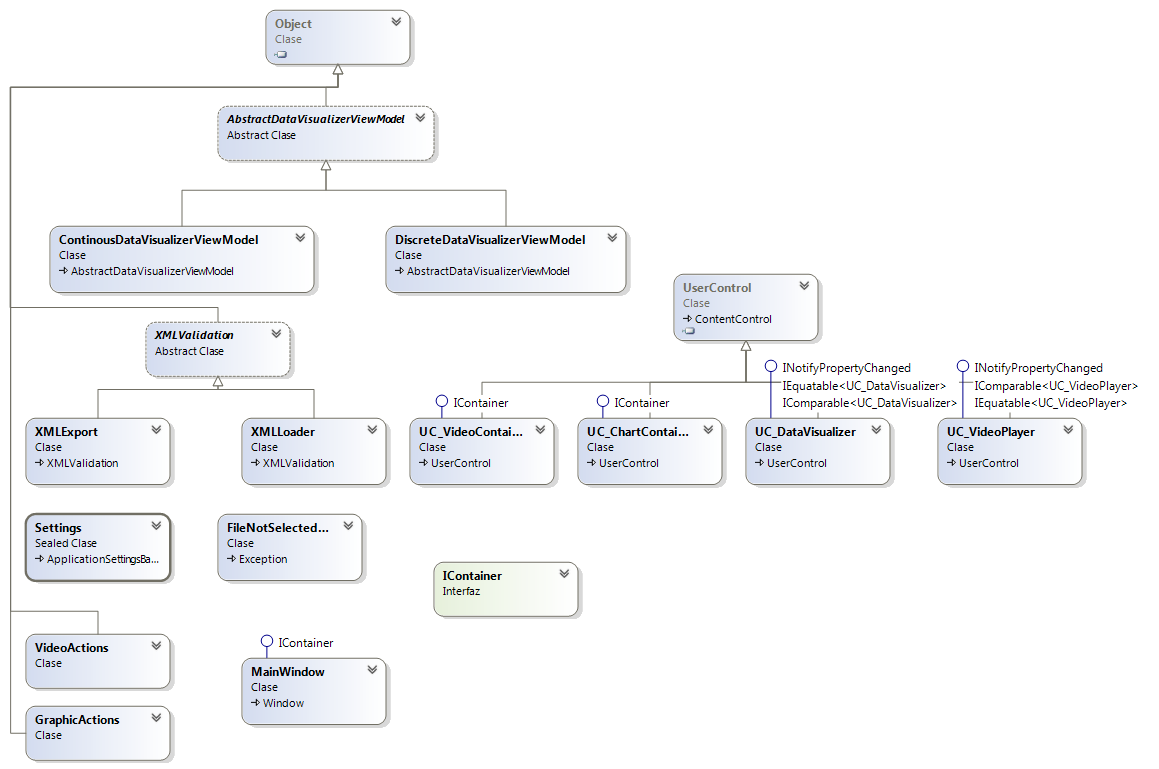
\includegraphics[width=1.2\linewidth]{./Figures/ClassDiagram}
	\caption[Diagrama de clases compacto]{Diagrama de clases compacto}
	\label{fig:ClassDiagram}
\end{figure}

\subsubsection{AbstractDataVisualizerViewModel}
Clase abstracta que describe e implementa todos los m\'etodos y propiedades que han de tener todos los ViewModels. Es decir,
define todo aquello que podr\'a ser cargado por un \emph{UC\_DataVisualizer}. Esta clase expone el m\'etodo
\emph{private PlotModel createModel(List<DataPoint> points)}
que todas sus clases han de implementar.

\subsubsection{ContinousDataVisualizerViewModel}
Subclase de \emph{AbstractDataVisualizerViewModel} que se especializa en tratar los datos cont\'inuos. 

\subsubsection{DiscreteDataVisualizerVIewModel}
Subclase de \emph{AbstractDataVisualizerViewModel} que se especializa en tratar los datos discretos.
Esta clase requiere de datos adicionales, los elementos del eje de ordenadas.

\subsubsection{XMLValidation}
Clase abstracta que sirve como base a todas aquellas clases que requieran de validar un XML contra un XSD.

\subsubsection{XMLExport}
Subclase de \emph{XMLValidation} que se encarga de gestionar todo lo relacionado con exportar un XML. Creaci\'on y
validaci\'on de intervalos y guardar a disco el paso o situaci\'on principalmente.

\subsubsection{XMLLoader}
Subclase de \emph{XMLValidation} que tiene como responsabilidad cargar los datos del XML, tanto obtener los datos
para mostrar en el \'arbol como de crear los ViewModels que despu\'es ser\'an utilizados por los \emph{UC\_DataVisualizer}.

\subsubsection{VideoActions}
Clase Singleton que proporciona los m\'etodos necesarios para gestionar los v\'ideos cargados.

\subsubsection{GraphicActions}
Clase Singleton que gestiona los \emph{UC\_ChartContainer}. A\~nadir, borrar, sincronizar rangos etc.

\subsubsection{UC\_VideoContainer}
Control de usuario derivado de \emph{UserControl} y que implementa
la interfaz \emph{IContainer}. Dispone de la interfaz y los m\'etodos necesarios para
gestionar los \emph{UC\_VideoPlayer} (a\~nadir, borrar etc) as\'i como unos controles globales
para controlar su reproducci\'on.

\subsubsection{UC\_ChartContainer}
Control de usuario derivado de \emph{UserControl} y que implementa la interfaz
\emph{IContainer}. Esta clase contiene la interfaz gr\'afica y los m\'etodos requeridos para gestionar
los \emph{UC\_DataVisualizer}. Representa una observaci\'on que dentro tiene sus propiedades.
Tambi\'en es importante a\~nadir que es \'esta clase la que se suscribe al evento que notifica
que el rango seleccionado ha cambiado, para poder inicial el proceso de sincronizaci\'on.

\subsubsection{UC\_DataVisualizer}
Control de usuario que se encarga de mostrar los datos de las propiedades y una de las funcionalidades
principales consiste en notificar a su padre (un \emph{UC\_ChartContainer}) de que el rango seleccionado ha cambiado.

Esta clase extiende a \emph{UserControl} e implementa las interfaces \emph{INotifyPropertyChanged},
\emph{IEquatable<T>} e \emph{IComparable<T>}. Es necesario implementar
esas interfaces para que el \'arbol rojo negro funcione correctamente, ya que requiere ordenar las instancias
de alguna manera. 

\subsubsection{UC\_VideoPlayer}
Control de usuario que se encarga de reproducir v\'ideos.

Al igual que \emph{UC\_DataVisualizer} extiende \emph{UserControl} 
e implementa las interfaces \emph{INotifyPropertyChanged},
\emph{IEquatable<T>} e \emph{IComparable<T>}. Los motivos de su implementaci\'on
son los mismos que en \emph{UC\_DataVisualizer}.

\subsubsection{IContainer}
Esta interfaz define aquellos m\'etodos que deben ser implementados por las clases que vayan a ser contenedores
de alg\'un tipo de dato.

\subsubsection{FileNotSelectedException}
Excepci\'on personalizada pensada para ser lanzada en los di\'alogos de apertura de ficheros.

\subsubsection{MainWindow}
Punto de entrada al programa. Al ser un contenedor de contenedores, concretamente de \emph{UC\_ChartContainer} y
\emph{UC\_VideoContainer}, tambi\'en implementa la interfaz \emph{IContainer}.

Esta clase, principalmente se encarga de realizar las llamadas a cargar los datos y añadir las observaciones
y el contenedor de v\'ideos.
   \chapter{Desarrollo}

\section{Qu\'{e} se ha hecho}
Se ha desarrollado una aplicaci\'{o}n que dados unos datos organizados
de cierta manera permite la visualizaci\'{o}n de los mismos y
la selecci\'{o}n de unos rangos para guardar y especificar que en ese rango de tiempo
est\'{a} sucediendo una acci\'{o}n determinada, ya sea un Paso o una Situaci\'on.

Los datos de entrada representan Observaciones y Propiedades. Cada observaci\'{o}n tiene una serie
de propiedades que son las que se visualizan. Estos datos, cuando fueron capturados, puede
que tengan uno o varios v\'{i}deos asociados. La visualizaci\'{o}n de los v\'{i}deos es completamente
optativa, y en caso de visualizarlos, van sincronizados con los gr\'{a}ficos a partir del instante que el 
usuario diga.

Es decir, en cada gr\'{a}fico habr\'{a} una l\'{i}nea de progreso para que sea f\'{a}cil determinar en que ciclo
de simulaci\'{o}n estamos \footnote{Un ciclo de simulaci\'{o}n es la unidad de tiempo elegida para la captura de datos, no
    necesariamente es un segundo.}.

Una vez hemos determinado cual es el problema ha resolver, se hace necesario tomar ciertas decisiones.
Desde un principio se sab\'ia que hab\'ia que programar en un entorno Windows, utilizando Visual Studio 2013.
La raz\'on de esta decisi\'on fue que el proyecto actual est\'a desarrollado utilizando Windows Forms, y el 
director del proyecto coment\'o que exist\'ia una intenci\'on de portarlo a WPF.

Pese a conocer a esa intenci\'on, hubo que valorar que merec\'ia m\'as la pena, si utilizar WPF, una tecnolog\'ia moderna
en la que Microsoft est\'a poniendo todo su empe\~no, o bien Windows Forms, que es un viejo conocido del desarrollo
.NET con un camino muy largo de desarrollo.

Para decidir de la manera m\'as objetiva posible, se confeccion\'o la tabla \ref{ComparativaWPF} en la que se sit\'uan 
las caracter\'isticas de cada tecnolog\'ia. La tabla es una elaboraci\'on propia confeccionada a partir de una comparativa
online \cite{WPFvsWinForms:Comparative}.

\begin{table}[H]
	\begin{center}
		\rowcolors{1}{lightgray}{} %\rowcolors{<starting row index>}{<odd row color>}{<even row color>}
		\begin{tabular}{|p{5cm} | p{4cm} | p{4cm}|}
			\rowcolor{darkgray}                         & \color{white}Windows Forms               & \color{white}WPF \\
			Formularios y controles                     & Si                                       & Si \\
			Documentos en pantalla                      & Si                                       & Si \\
			Documentos de formato fijo (XPS, PDF)       & No                                       & Si \\
			Im\'{a}genes                                & No                                       & Si \\
			V\'{i}deo y audio                           & No                                       & Si \\
			Gr\'{a}ficos 2D                             & No                                       & Si \\
			Gr\'{a}ficos 3D                             & No                                       & Si \\
			Interfaz compatible con altas resoluciones  & No, basada en BMP                        & Si, basada en vectores \\
			Creaci\'{o}n de la interfaz                 & Arrastrando y soltando los elementos     & Interfaz declarativa tipo XML \\
			Multilenguaje                               & Mediante archivos de recursos, f\'{a}cil y bien documentado & Mediante DLLs sat\'{e}lite, poco documentado y las herramientas aun no est\'{a}n listas para un entorno de producci\'{o}n. \\
			\hline
		\end{tabular}
	\end{center}
	\caption[Comparativa Windows Forms y WPF]{Comparativa Windows Forms y WPF}
	\label{ComparativaWPF}
\end{table}

C\'omo puede observarse, Windows Forms se ha quedado obsoleto para un desarrollo de aplicaciones moderno.
Pese a todo, WPF, tiene algunos puntos d\'ebiles. Entre ellos, el soporte multilenguaje, y que es un proyecto
mucho menos maduro, ya que fue lanzado en 2006 junto con .NET Framework 3 \cite{WPF:Overview}. Windows Forms,
por su parte se present\'o junto con la primera version de .NET Framework, en 2002.

Esta elecci\'on condiciona el resto de decisiones que fueron tomadas, ya que las bibliotecas gr\'aficas
de Windows Forms no son compatibles con WPF. Existe una capa de compatibilidad en la que es posible embeber dentro
de un host WPF un control Windows Forms, pero no es recomendable, ya que no deja de ser una capa de compatibilidad y
no es posible sacarle toda la potencia a Windows Presentation Foundation.

Una de las primeras decisiones que se tomaron, y adem\'as sin demasiado debate, fue que tipo de interfaz se deseaba.
Se eligi\'o una interfaz tipo IDE, con ventanas acoplables, tal y como se ha detallado en el cap\'itulo de Antecedentes.

En este caso en concreto no hubo que buscar mucho, ya que no hay mucho donde elegir. La biblioteca seleccionada
fue AvalonDock.

AvalonDock es una biblioteca escrita \'integramente para WPF, con soporte para MVVM. Permite todo lo que se espera
de un proyecto como ese: Ventanas acoplables a los lados, mover pesta\~nas etc, fue curioso que durante desarrollo se descubri\'o
un bug en el software.

Dicho bug, lanzaba una excepci\'on cuando un elemento ``acoplable", que ten\'ia un Men\'u superior, al ponerlo
en una pesta\~na, al cambiar de pesta\~na fallaba. El bug ya estaba reportado, pero aun as\'i se le proporcion\'o
al desarrollador m\'as informaci\'on sobre el bug \footnote{\url{https://avalondock.codeplex.com/discussions/429063}}.

Antes de explicar como es la interfaz que se ha dise\~nado, primero hay que saber como trabaja internamente
AvalonDock y como se usa para poder crear esas pesta\~nas y ventanas acoplables.

Explicado de manera muy sencilla, AvalonDock se compone de cuatro partes principales: el \emph{DockingManager},
el \emph{LayoutPanel}, el \emph{LayoutAnchorablePane}, y el \emph{LayoutAnchorable}.
Tambi\'en tiene otros elementos pero no han sido usados en este proyecto.

\paragraph{DockingManager:} Es el n\'ucleo de AvalonDock, donde todos los elementos WPF son a\~nadidos, necesario
siempre para poder trabajar con AvalonDock.

\paragraph{LayoutPanel:} Este elemento organiza todos los hijos, poniendo un separador entre ellos, establecido
usando la propiedad \emph{Orientation}.

\paragraph{LayoutAnchorablePane:} Estos elementos son la clave. Ya que es el panel que permite que los objetos
\emph{LayoutAnchorable} pueden ser arrastrados, puestos en pesta\~nas, lado a lado etc.

\paragraph{LayoutAnchorable:} Estos elementos siempre deben ir dentro de un \emph{Pane}, bien \emph{LayoutAnchorablePane}
bien \emph{LayoutDocumentPane} que no ha sido explicado. Estos elementos son los que pueden reorganizarse como uno quiera,
anclarse a un lado, poner que se oculten etc. Y dentro pueden tener aquello que se desee.

Por tanto, para tener una instancia funcional de AvalonDock, tendremos que tener un \emph{DockingManager} y un
\emph{LayoutRoot} dentro de ese dockingmanager. Y dentro de ese \emph{LayoutRoot} un \emph{LayoutAnchorablePane}.

Una vez tenemos eso, a\~nadir a un \emph{LayoutAnchorable} un elemento es muy sencillo, no hay mas que a\~nadirlo dentro de la
propiedad Content. Y para a\~nadir ese \emph{LayoutAnchorable} al \emph{LayoutAnchorablePane} hay que a\~nadirlo a la colecci\'on
de hijos. En la Figura \ref{AnadirHijoAvalonDock} se puede ver un ejemplo de como se a\~nade un \emph{UC\_DataVisualizer} a 
AvalonDock.

\begin{figure}[h]
    \begin{lstlisting}[tabsize=2, language=C, numbers=left, showspaces=false, breaklines=true]
    public void addToAnchorablePane(UserControl objectToAdd, string Title)
    {
        UC_DataVisualizer datav = (UC_DataVisualizer)objectToAdd;
        LayoutAnchorable doc = new LayoutAnchorable();
        doc.Title = Title;
        doc.Content = datav;
        mainPanelChartContainer.Children.Add(doc);

    }
    \end{lstlisting}
    \caption[Adici\'on de elemento a AvalonDock]{Adici\'on de elemento a AvalonDock}
    \label{AnadirHijoAvalonDock}
\end{figure}

Una vez conocemos el funcionamiento de AvalonDock, podemos pasar a hablar de la interfaz dise\~nada.
La estructura que se ha dise\~nado es un ``workbench", con un panel lateral en el que se pueden visualizar las observaciones
y propiedades disponibles despu\'es de haber cargado un fichero XML. Cuando se hace doble click sobre un elemento
de ese \'arbol de propiedades y observaciones, el software sabe si se ha pinchado en una propiedad o en una observaci\'on.
Si se quiere saber que sucede cuando se pincha en cada uno de ellos, todo esto est\'a mejor explicado en la secci\'on de
Captura de requisitos, en los casos de uso extendidos.

Cuando se cargan los datos que se desean, es decir, que se visualizan, como puede verse en la
Figura \ref{fig:EjemploObservacion} se muestran organizados por observaciones. Y dentro de cada
observaci\'on las propiedades que han sido cargadas. Las ventanas pueden organizarse como se quiera, ponerlas lado a lado,
reordenar las pesta\~nas, colapsarlas a un lateral, dejarlas como ventanas flotantes etc. 
La \'unica limitaci\'on intencionada es que una propiedad no puede acoplarse a una observaci\'on a la que no pertenece,
para evitar confusiones.

\begin{figure}[h]
	\centering
	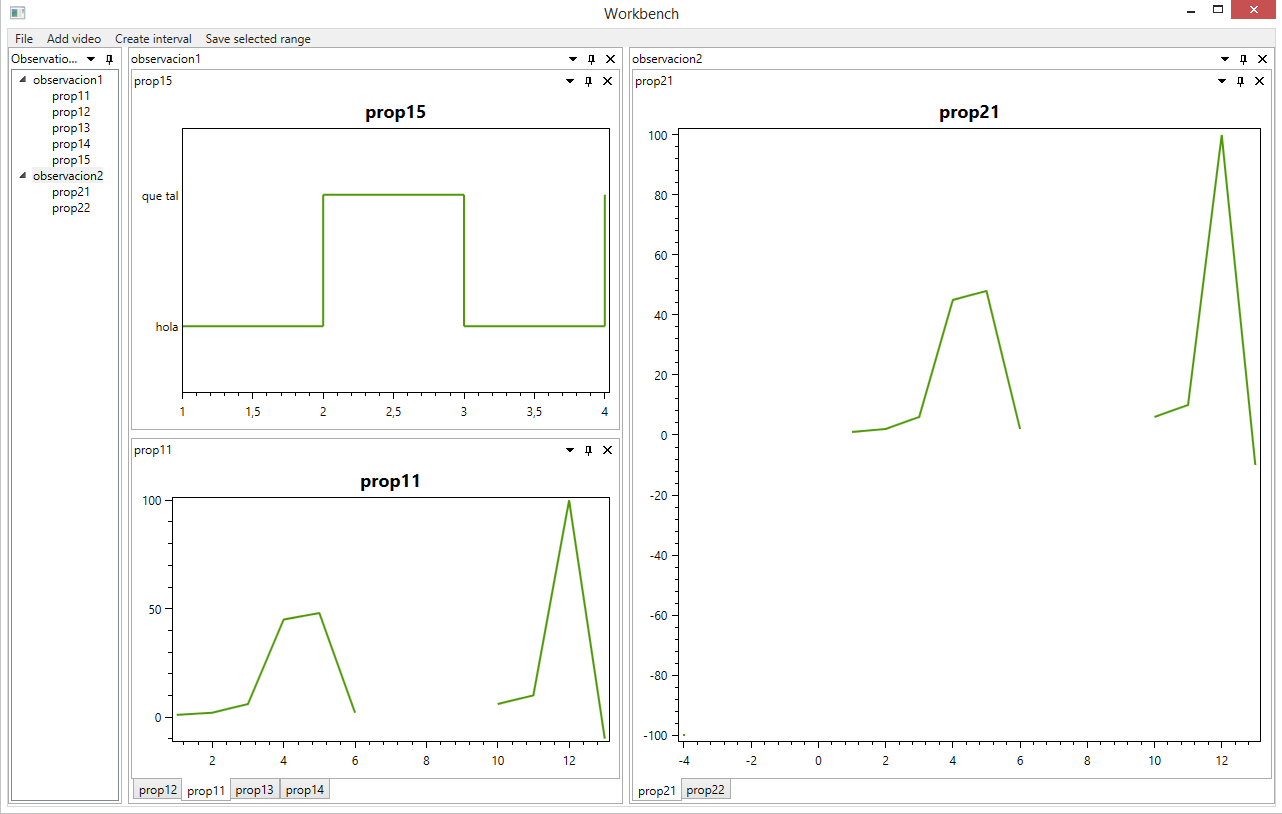
\includegraphics[width=0.9\linewidth]{./Figures/Capturas/EjemploObservacion.PNG}
	\caption{Ejemplo de visualizaci\'on de propiedades}
	\label{fig:EjemploObservacion}
\end{figure}

Despu\'es de escoger el tipo de organizaci\'on de ventanas, era necesario elegir como iban a mostrarse los gr\'aficos en pantalla.
Para el sistema de gr\'aficos no hubo problemas a la hora de encontrar distintas librer\'ias, pero si que fue un 
problema encontrar uno que cumpliera las siguientes caracter\'isticas.

\begin{itemize}
	\item Permitir mostrar gr\'{a}ficos cont\'{i}nuos y discretos, y estos \'{u}ltimos tanto num\'{e}ricos como por categor\'{i}as.
	\item Permitir la selecci\'{o}n de rangos con el rat\'{o}n.
	\item Permitir mostrar el progreso del v\'{i}deo asociado. Bien sin programar la funci\'{o}n o al menos que fuese f\'{a}cilmente programable.
\end{itemize}

Se descartaron todas las bibliotecas de pago, como pueden ser Telerik, SciChart, Visiblox, etc. por ser demasiado caras
y porque se decidi\'o utilizar en la medida de lo posible tecnolog\'ias libres y gratuitas. Entre las bibliotecas
gratuitas, destacaron tres por encima de todas. Las capacidades nativas de WPF,
WPF toolkit, desarrollada por Microsoft, y OxyPlot.

Los gr\'aficos 2D integrados en WPF son muy simples de utilizar, con una est\'etica muy minimalista, de colores planos.
Lamentablemente, la selecci\'on de rangos, y mostrar leyendas en los ejes X e Y no eran tareas triviales, por lo que
se descart\'o al poco de iniciar el desarrollo.

WPF toolkit fue la siguiente librer\'ia en pasar la prueba. Se integra a la perfecci\'on 
en Visual Studio y muestra unos gr\'aficos muy profesionales de una forma
muy simple, pero desafortunadamente, no existe una manera sencilla de seleccionar un rango.

OxyPlot, por su parte, es un proyecto comunitario en constante desarrollo. Con decenas de ejemplos online en su web
oficial fue muy sencillo crear un prototipo funcional con todos los gr\'aficos requeridos, con las leyendas en los ejes
y los t\'itulos. Conseguir la selecci\'on de un rango conllev\'o algo m\'as de tiempo de desarrollo.

Para crear un gr\'afico es tan f\'acil como crear en el XAML un elemento \emph{<oxy:PlotView />} que va a ser el 
elemento a contener el gr\'afico. Despu\'es, \'unicamente hay que a\~nadir un \emph{PlotModel}, que es la
clase que contiene tanto los puntos, el titulo del gr\'afico, los ejes etc. Lo mejor en estos casos es un ejemplo.
En la Figura \ref{CreacionPlotModel}, se ve el m\'etodo de creaci\'on de un \emph{PlotModel} para un visualizador de datos
discreto.

\begin{figure}[h]
    \begin{lstlisting}[tabsize=2, language=C, numbers=left, showspaces=false, breaklines=true]
    protected override PlotModel createModel(List<DataPoint> points)
    {
        var plotModel = new PlotModel();
        var functionSeries = new StairStepSeries();
        var categoryAxis = new CategoryAxis();
        
        categoryAxis.Position = AxisPosition.Left;
        categoryAxis.AxislineStyle = LineStyle.Solid;
        categoryAxis.MinorStep = 1;
        categoryAxis.TickStyle = TickStyle.None;
        categoryAxis.Labels.AddRange(Labels);
        plotModel.Axes.Add(categoryAxis);
        functionSeries.Points.AddRange(points);
        plotModel.Series.Add(functionSeries);
        plotModel.Title = Title;
        Points = functionSeries.Points;
        return plotModel;
    }
    \end{lstlisting}
    \caption[Creaci\'on PlotModel]{Creaci\'on PlotModel}
    \label{CreacionPlotModel}
\end{figure}

La selecci\'on de un rango,se hace a\~nadiendo al \emph{PlotModel} un elemento \emph{RectangleAnnotation}.
Para actualizar el valor de inicio y fin de ese rango, hay que suscribirse a tres eventos, ya que una selecci\'on
de rango es la combinaci\'on de tres eventos: hacer click, arrastrar, y dejar de hacer click. Cuando se pincha,
se establece el lugar de inicio de selecci\'on, y mientras se va moviendo el rat\'on, si el bot\'on izquierdo
del rat\'on est\'a presionado, entonces se va actualizando el rango seleccionado. Y cuando se deja de pinchar,
termina el proceso.

En los primeros prototipos, en cada gr\'afico pod\'ia seleccionarse un rango diferente, pero era algo inconsistente, ya
que cuando llegase la hora de guardar los rangos, ¿Cual se usar\'ia? Por lo que fue necesario continuar un poco con la 
investigaci\'on para ver como podr\'ia un hijo notificar a su padre de que ha cambiado, para que ese padre notifique a todos
sus hijos para sincronizarse.

La primera aproximaci\'on, y posiblemente la peor de todas, era realizar un \emph{polling}, es decir, cada, por ejemplo, 60 ms,
preguntar a cada elemento si ha cambiado, y si alguno lo ha hecho, utilizar ese valor para poner ese rango en los dem\'as 
gr\'aficos. Este enfoque, tiene diversos problemas, pese a que los gr\'aficos est\'an guardados en \'arboles rojo-negro
\footnote{\url{https://www.cs.auckland.ac.nz/~jmor159/PLDS210/red\_black.html}}
\footnote{\url{https://www.cs.princeton.edu/courses/archive/fall08/cos226/lectures/10BalancedTrees-2x2.pdf}},
no tiene sentido recorrer el \'arbol constantemente, y si se encuentra un elemento, habr\'ia que recorrer cada observaci\'on cargada,
y para cada observaci\'on todas las propiedades cargadas actualmente. Eso,
conllevar\'ia un coste de O(2*n*m) siendo ``n" \ el n\'umero de observaciones cargadas y ``m" \ el n\'umero de propiedades.

La otra soluci\'on, es implementar la interfaz \emph{INotifyPropertyChanged}. Utilizando esta interfaz, se expone un 
nuevo evento, llamado \emph{PropertyChanged} al que otros objetos se pueden suscribir para estar a la escucha.

De esta manera, cada vez que se a\~nada un nuevo gr\'afico, el contenedor de gr\'aficos se suscribe a ese evento para todos
sus hijos. De esta manera, cuando el rango seleccionado cambie, ser\'a ese hijo el que notifique al padre, que iniciar\'a
el proceso de sincronizado, tanto con sus hijos como con sus hermanos (el resto de observaciones cargadas).

Para la visualizaci\'on de v\'ideos no hubo mucho problema, y se utilizaron los
propios componentes de WPF, que cumpl\'ian todas las necesidades.

Por su parte, cargar los datos no fue demasiado problema una vez se decidi\'o cual iba a ser el formato de los
ficheros XML.

Se barajaron dos posibilidades. La primera, que por cada instante de simulaci\'on se guardaran las observaciones
que est\'an teniendo lugar, y los valores de las propiedades que tienen en ese instante, tal y como
se puede ver en la Figura \ref{Estructura XML1}.

Este formato, a la vista parece bueno, ya que se pordr\'ia construir los gr\'aficos instante a instante,
todos a la vez. Pero, ¿Y si se quiere obtener el valor de una propiedad en concreto para mostrar todo 
el gr\'afico de golpe? No se obtiene de manera directa, ya que habr\'ia que ciclar a trav\'es de todos los nodos
instante, y a trav\'es de todos los nodos observaci\'on, buscando la propiedad deseada.

Tambi\'en hay que tener en cuenta, que en distintas observaciones puede haber propiedades que tengan el mismo nombre, 
aumentando la complejidad de la consulta LINQ (m\'as adelante se hablar\'a de este tema).

\begin{figure}[h]
    \lstinputlisting[tabsize=2, language=XML, numbers=left]{./Attachments/Adjunto1.xml}
    \caption[Estructura XML 1]{Estructura XML 1}
    \label{Estructura XML1}
\end{figure}

La segunda opci\'on barajada, toma un enfoque distinto., tal y como se puede
ver en la Figura \ref{Estructura XML2}. Los datos se agrupan por observaci\'on, con las observaciones teniendo sus propiedades,
y estas \'ultimas sus instantes. De esta manera, de un simple vistazo podemos determinar todos los valores que va a tomar
una propiedad de una observaci\'on en concreto, sin ning\'un tipo de consulta compleja.
En el nodo \emph{<data>} se ha a\~{n}adido un nuevo atributo \emph{instantLength} que 
determina la longitud de un instante. 

Por ejemplo, en la propiedad \emph{prop14} se ve que los instantes no son consecutivos, por lo que el sistema sabe que el 
gr\'{a}fico no debe ser cont\'inuo en ese punto, es decir, desde el punto (1, 4) no debe unirse al 
(3, 5). Esto es \'{u}til para saber si una propiedad esta sucediendo o no.

\begin{figure}[h]
    \lstinputlisting[tabsize=2, language=XML, numbers=left]{./Attachments/Adjunto2.xml}
    \caption[Estructura XML 2]{Estructura XML 2}
    \label{Estructura XML2}
\end{figure}

Otro de los problemas fundamentales que se tuvieron, fue como guardar los datos. Debido a que de momento el software
aqu\'i presentado va a ser completamente independiente, hab\'ia que buscar una manera de compartir los datos
que implicara el menor n\'umero de cambios posibles en el sistema ya creado por el grupo de investigaci\'on.

Se barajaron varias posibilidades, como por ejemplo, las bases de datos relaciones, pero este sistema requerir\'ia
de una estructura compleja para guardar unos datos bastante sencillos. Ya que del modelo de dominio, se infiere que m\'inimo,
iba a haber 4 tablas para poder guardar los datos correctamente. Adem\'as, los datos no iban a ser f\'acilmente 
comprensibles por humanos, ya que ser\'ian un amasijo de n\'umeros guardados en tablas que ser\'ian dif\'iciles de
relacionar entre ellas de manera sencilla.

Es por ello que se valor\'o la posibilidad de utilizar las bases de datos no relacionales, que est\'an tan de moda
\'ultimamente. Concretamente, el producto sometido a pruebas fue MongoDB. Es una base de datos NO-SQL en la que los
datos se guardan en formato de ``documentos", no tablas. Internamente, se guardan en formato BSON, que no deja de ser
un JSON binario \footnote{Especificaci\'{o}n JSON: \url{http://json.org/}}. Ofrece un gran rendimiento, adem\'as
de unos datos mejor organizados para esta tarea, con elementos que tienen arrays, y cada elemento atributos etc.

Finalmente se opt\'o por descartarlo tambi\'en, ya que a\~nad\'ia mayor complejidad, ``oscuridad" \ y requisitos a la 
implementaci\'on. Ya que habr\'ia que tener instalada una base de datos MongoDB, as\'i como los conectores para
C\#.

As\'i que se decidi\'o ir por el camino de en medio y elegir un est\'andar que no requiriera de software adicional,
que fuese soportado de manera nativa por el lenguaje de programaci\'on y adem\'as f\'acilmente comprensible por
humanos. El elegido fue XML m\'as la biblioteca LINQ To XML incluida por defecto en .NET Framework. 

XML es un est\'andar recomendado por la W3C \cite{XML:Specification}, y la versi\'on actual es la 1.0 quinta edici\'on.
Por si mismo, XML no aporta ning\'un tipo de ventaja adicional respecto a las otras opciones, excepto el que no se
requiere de software adicional para compartir los datos de una aplicaci\'on a otra, y que
se pueden crear esquemas XSD para validar esos datos de manera muy sencilla. 
Lo que realmente marca
la diferencia es LINQ To XML.

LINQ To XML es una extensi\'on de la biblioteca LINQ (Language Integrated Query), que permite hacer consultas
similares a SQL a estructuras de datos .NET. 

En el ejemplo de la Figura \ref{Consulta LINQ}, extra\'ido de mi propio c\'odigo, se obtienen las propiedades de
una determinada observaci\'on.
Concretamente, este c\'odigo se ha utilizado a la hora de cargar el \'arbol lateral
de observaciones y propiedades.

\begin{figure}[h]
	\begin{lstlisting}[tabsize=2, language=C, numbers=left, showspaces=false, breaklines=true]
		internal List<string> getPropertiesOf(string observation)
        {
            List<string> listProperties = null;
            
            IEnumerable<XElement> properties =
                from prop in xml.Descendants("property")
                where (string)prop.Parent.Attribute("name") == observation
                select prop;
            
            listProperties = addElements(properties);
            return listProperties;
        }
	\end{lstlisting}
	\caption[Consulta LINQ]{Consulta LINQ}
	\label{Consulta LINQ}
\end{figure}

Una vez elegido el m\'etodo de guardado de datos, se llego a la tesitura de elegir una estructura para el XML.
Las dos opciones valoradas fueron las siguientes.

Una cosa interesante y que adem\'as no se ped\'ia desde el principio, era si 
ten\'ia sentido implementar procesamiento paralelo o procesos en segundo plano. El 
procesamiento paralelo finalmente no tiene sentido implementarlo ya que no hay tareas
que puedan separarse en subtareas para que cada ``trabajador" \ pueda procesar por su
cuenta. En cambio, al no conocerse el tama\~no m\'aximo de entrada, se ha decidido
implementar un \emph{BackgroundWorker} a la hora de crear un intervalo, y a la hora
de guardar en disco el paso o la situaci\'on.

Se ha tomado esta decisi\'on porque si el guardar los datos se hace en el hilo principal
de ejecuci\'on, dependiendo de la cantidad de datos, podr\'ia bloquear la interfaz y
de esta manera el software es mucho m\'as escalable. Bien es
verdad que un procesador moderno es capaz de procesar unos 50 millones de operaciones por
segundo, y no se cree que la entrada, ni la salida vaya a ser tan grande.

A la hora de cargar datos, no se ha implementando el \emph{BackgroundWorker}
porque en la aplicaci\'on no se puede realizar ninguna acci\'on hasta que los datos est\'an 
listos. Pese a todo, al cargar el XML no se cargan todos los datos, sino que se obtienen \'unicamente
los nombres de las propiedades y las observaciones. Los datos en si se cargan bajo demanda, para optimizar la memoria
utilizada del propio software haci\'endolo mas \'agil al mismo tiempo, ya que de esta manera el software no
tiene que preocuparse de que datos est\'an cargados y cuales no, ya que todo aquello que est\'a cargado debe
procesarse.

Otras de las cosas que se implementaron a \'ultima hora fue la posibilidad de guardar m\'ultiples
intervalos en un mismo Paso o Situaci\'on, ya que en palabras del director del TFG: ``No todo lo que est\'a 
relacionado sucede \'unicamente durante un intervalo de tiempo". Para hacer frente a esta nueva funcionalidad
hubo dos enfoques principales. El primero de ellos, consist\'ia en que cada vez que se le diera a guardar
intervalo, el software preguntara si se quer\'ian a\~nadir intervalos mas tarde. Cuando se pinchara que no
se mostrar\'ia el di\'alogo de guardar y se guardar\'ia a disco.

La otra opci\'on, era separar las dos acciones, por un lado, crear los intervalos, y por otro lado guardar a disco.
Finalmente se utiliz\'o la segunda manera porque se cree de que es mas intuitivo tener dos acciones separadas
que se sabe bien que realiza cada una, con un flujo de trabajo claro, a tener una \'unica acci\'on, que dependiendo
de la acci\'on del usuario haga una cosa u otra. 

En cuanto a las cuestiones de dise\~no, tal y como se ha contado previamente en el cap\'itulo
de An\'alisis y dise\~no se ha realizado de manera iterativa, mejorando el dise\~no sprint tras sprint,
ya que creo que hacer un buen dise\~no desde el principio sin conocer en su totalidad que ha de hacerse
es un error y una p\'erdida de tiempo.

Por ejemplo, al principio, la clase \emph{GraphicsActions} conten\'ia una lista con todos los 
\emph{UC\_DataVisualizer}. Este
acercamiento se eligi\'o al principio ya que era el m\'as simple para conseguir el objetivo del mes: mostrar datos.

Posteriormente, se hizo necesario guardar tambi\'en los \emph{UC\_ChartContainer}, ya que las propiedades estaban agrupadas por
observaci\'on. Por lo tanto \emph{GraphicsActions} pas\'o a tener un \emph{HashMap} teniendo como clave el nombre de la 
observaci\'on
y como contenido una lista de \emph{UC\_DataVisualizer}. Pero ese dise\~no entra en conflicto con uno de los principios
SOLID que se explicar\'an m\'as adelante. Por lo que \emph{GraphicsActions} ahora es un repositorio de 
\emph{UC\_ChartContainer},
y cada \emph{UC\_ChartContainer} contiene una lista de los\emph{ UC\_DataVisualizer} que 
pertenecen a esa observaci\'on y un \emph{HashSet}
con los nombres de las propiedades, para poder obtener en tiempo constante si ya estaban cargados, ya que solo se pueden cargar
una \'unica vez.

En la \'ultima iteraci\'on, se decidi\'o sustituir el \emph{HashSet} y la lista por un \'arbol rojo negro. Ya que permite
inserci\'on, b\'usqueda y eliminaci\'on en tiempo O(ln n) frente al O(n) de las listas. 
Adem\'as un \'arbol rojo negro, s\'olo permite que existe una vez el mismo objeto en el \'arbol.

\section{Gesti\'{o}n del c\'{o}digo fuente}
Hasta ahora no se ha hablado de algo que bien no es parte del desarrollo, pero que igualmente es importante.

Hoy en d\'ia, todo proyecto debe tener alg\'un tipo de gesti\'on del c\'odigo fuente, para evitar p\'erdida de datos, 
poder volver a versiones anteriores y tener una mejor noci\'on de que se ha cambiado si es un proyecto colaborativo.

En este caso, al ser un proyecto realizado por una \'unica persona, parec\'ia razonable utilizar alg\'un otro tipo
de sistema. Ya que Git, CVS o Subversion son piezas de software muy potentes y usadas a gran escala, pero tinen
una curva de aprendizaje bastante pronunciada.

Por tanto se valor\'o la posibilidad de utilizar Dropbox como sistema de gesti\'on y sincronizado del c\'odigo fuente.
Pero los problemas no tardaron en aflorar con cuestiones del tipo:

¿Qu\'e pasar\'ia si se quiere volver a una versi\'on que hice hace 20 d\'ias? ¿C\'omo se crea un trabajo derivado a partir
de una versi\'on concreta? Por lo que finalmente se decidi\'o usar GIT, ya que incluso con la curva de aprendizaje,
es una herramienta muy potente y \'util, en la que se puede ver f\'acilmente qu\'e se hizo cierto d\'ia, o volver sin 
ning\'un problema a lo que se hizo ayer, o a lo que se hizo el primer d\'ia de proyecto.

Crear una nueva rama de desarrollo a partir de cualquier versi\'on es muy \'util y pr\'actico, por ejemplo, para
realizar pruebas experimentales sin romper el trabajo estable que se ha realizado hasta el momento. Tambi\'en
ha sido fruto de diversos problemas, pero nada que el manual oficial o stackoverflow no pudieran
resolver en unos minutos.

\section{Creaci\'{o}n de la documentaci\'{o}n}
Aunque esta secci\'{o}n pueda parecer una elecci\'{o}n obvia, trajo bastantes quebraderos de cabeza. Por un lado
se quer\'{i}a algo que no requiriera
de un estudio previo de 3 meses, que fuese lo suficientemente potente, que su rendimiento no decreciera seg\'{u}n aumentaban las 
p\'{a}ginas, y desde luego,
que pudiera editar tanto desde Windows, como Linux.

C\'{o}mo el proyecto lo estaba realizando en Windows y para Windows, Microsoft Office, parec\'{i}a la elecci\'{o}n obvia. Un 
producto potente muy bien integrado
en Windows, que permite crear documentos muy vistosos de manera muy sencilla. 
Pese a s\'olo tener versiones oficiales de Windows y Mac OSX en Linux
funciona razonablemente bien utilizando WINE. Pero cu\'anto m\'as largo es un documento, el programa cada vez reacciona
m\'as despacio, siendo complicado trabajar con documentos largos o con un dise\~no complejo.

Tambi\'en se valor\'o la posibilidad de usar LibreOffice u OpenOffice, por ser multiplataforma, pero adolecen
de las mismas limitaciones que Office. En ambas suites la colocaci\'on de im\'agenes y tablas puede ser como poco,
intrincado, pudiendo destrozar por completo el dise\~no del documento por querer mover medio cent\'imetro una tabla a la
derecha.

La \'ultima opci\'on valorada, y en la que este documento est\'a escrito ha sido \LaTeX.
Software de composici\'{o}n de textos creado por Donald E. Knuth \footnote{\url{http://www-cs-faculty.stanford.edu/~uno/}} 
muy popular entre los cient\'{i}ficos. Ofrece una manera similar de crear documentos a HTML 
aunque deber\'{i}a decirse al rev\'{e}s, ya que \LaTeX es bastante m\'as antiguo.

Para sacarle todo el partido se requiere un buen editor, con resaltado de sintaxis y autocompletado, 
la opci\'on elegida ha sido TexStudio, un
software de c\'{o}digo abierto que ofrece todo tipo de facilidades, multiplataforma.

All\'a donde el resto de software de edici\'on de textos fracasa, LaTeX resalta. Los ficheros, al ser de texto plano,
pueden integrarse en el software de control de versiones. El escritor puede abstraerse completamente del formato
y centrarse en escribir.

Tambi\'en es necesario decir, que pese a que la documentaci\'on ha sido escrita principalmente en LaTeX, algunas figuras
y gr\'aficos han sido creados con otras herramientas, entre ellas LibreOffice y Microsoft Word 2010.

   \chapter{Verificaci\'{o}n y evaluaci\'{o}n}
En este cap\'itulo se detallar\'an las pruebas
que se han llevado a cabo para verificar que el software
cumple todos los requisitos correctamente.

Las pruebas representan los comportamientos que debe
tener la aplicaci\'on, es decir, lo que se prueban son los
casos de uso y subcasos de uso, no si cada m\'etodo
realiza de forma correcta su tarea.

\section{Cargar XML}

\subsection{Preparaci\'on de las pruebas}
Para poder probar este comportamiento no se requiere de ninguna preparaci\'on 
especial.

\subsection{Cargar XML v\'alido nada m\'as abrir la aplicaci\'on}
Se prueba el comportamiento que debe tener la aplicaci\'on al cargar
un XML para empezar a trabajar, lo que se conoce como un arranque en fr\'io.

\paragraph{Resultado esperado}
Todos los datos cargados en la aplicaci\'on eliminados, 
tanto intervalos creados, como visualizadores de datos,
contenedores... todo debe haberse borrado de memoria volviendo a un estado inicial
de la aplicaci\'on.

\paragraph{Resultado obtenido}
Todos los datos se han borrado excepto los elementos del \'arbol de observaciones
y propiedades. 

\paragraph{Acciones realizadas}
Modificado el m\'etodo de cargar XML para limpiar tambi\'en los elementos del
\'arbol.

\subsection{Cargar XML v\'alido cuando ya haya un XML cargado}
Esta prueba contempla dos situaciones, 
ya que este comportamiento se da cuando hay
hay un XML cargado pero no se ha hecho nada, como cuando hay un XML cargado justo
despu\'es de guardar un paso o situaci\'on a disco.

\paragraph{Resultado esperado}
Todos los datos cargados en la aplicaci\'on eliminados, 
tanto intervalos creados, como visualizadores de datos,
contenedores... todo debe haberse borrado de memoria volviendo a un estado inicial
de la aplicaci\'on.

\paragraph{Resultado obtenido}
Todos los datos se han borrado.

\paragraph{Acciones realizadas}
Ninguna.

\subsection{Cargar XML v\'alido habiendo un XML cargado y con uno o varios intervalos guardados}
Esta prueba contempla el hecho de cargar un XML cuando ya hemos creado uno o varios
intervalos listos para ser guardados

\paragraph{Resultado esperado}
Todos los datos cargados en la aplicaci\'on eliminados, sobre todo dando mucha importancia a
que se eliminen los intervalos.

\paragraph{Resultado obtenido}
Todos los datos se han eliminado correctamente.

\paragraph{Acciones realizadas}
Ninguna por obtener el resultado esperado.

\subsection{Cargar un XML no v\'alido}
Se utiliza para comprobar si la funci\'on de validaci\'on funciona correctamente.

\paragraph{Resultado esperado}
Se mostrar\'a un error informando de que el XML que se ha intentado cargar
no valida contra el XSD.

\paragraph{Resultado obtenido}
El archivo se valida e intenta cargarse produciendo una
excepci\'on.

\paragraph{Acciones realizadas}
Se revisa tanto el c\'odigo de validaci\'on como el XSD para descubrir
d\'onde estaba el fallo. Finalmente se descubri\'o que el fallo estaba en el
XSD por lo que se arregla para que valide correctamente.

\section{Crear intervalo}
\subsection{Preparaci\'on de las pruebas}
Para poder crear un intervalo es necesario tener cargado un XML, y adem\'as haber cargado,
al menos, una propiedad en el sistema y tener un rango seleccionado.

\subsection{Guardar el rango no habiendo ninguno guardado previamente}
Se probar\'a si guarda correctamente un rango cu\'ando no hay ninguno guardado de antes.
Aqu\'i se pone a prueba el comportamiento de cuando se van a guardar rangos que no entran
en conflicto con ninguno.

\paragraph{Resultado esperado}
El rango se guarda en la colecci\'on de intervalos a guardar en disco, y se 
muestra un mensaje informando de que se ha a\~nadido correctamente.

\paragraph{Resultado obtenido}
El resultado obtenido es el esperado, se ha a\~nadido correctamente y se muestra
el mensaje de informaci\'on

\paragraph{Acciones realizadas}
Ninguna al obtener el resultado esperado

\subsection{Guardar un rango que solape a otro previamente guardado}
Esta prueba contiene a su vez cuatro pruebas que han sido agrupadas, ya que un intervalo
se puede superponer a otro de cuatro maneras, tal y como se ve en la Figura \ref{fig:ModosSolapamiento}.

\begin{figure}[H]
\centering
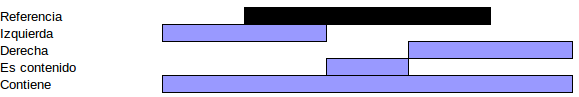
\includegraphics[width=0.9\linewidth]{./Figures/ModosSolapamiento.png}
\caption{Modos solapamiento}
\label{fig:ModosSolapamiento}
\end{figure}

El cuadrado negro representa el intervalo que est\'a guardado en el sistema, y 
los azules-lilas representan el que va a intentarse guardar.

\paragraph{Resultado esperado}
Las cuatro veces que intenten guardarse esos intervalos debe salir un mensaje informando
de que el intervalo a guardar solapa con alguno previamente guardado, y no debe
guardarse.

\paragraph{Resultado obtenido}
Para esos cuatro casos se obtiene el resultado esperado, pero en el caso extremo
en el que el intervalo guardado y el intervalo a guardar son iguales se guarda, dando
lugar a incongruencias. Hay que tener en cuenta que en el caso de empezar y acabar
en el mismo punto es la situaci\'on de ``contiene".

\paragraph{Acciones realizadas}
Se ajustan las comprobaciones, se cambian los ``<" \ y ``>" \ por ``$\leq$" \ y ``$\geq$".

\subsection{Guardar un intervalo vac\'io}
Lo que se prueba aqu\'i es que no se pueda guardar un intervalo vac\'io, ya que ser\'ia
llenar el XML resultante con etiquetas vac\'ias. Para probar se seleccionar\'a un rango
vac\'io y se pinchar\'a en crear intervalo.

\paragraph{Resultado esperado}
Un mensaje de advertencia indicando que es necesario seleccionar un rango, y
el intervalo no se guardar\'a.

\paragraph{Resultado obtenido}
No se muestra nada y se guarda el intervalo

\paragraph{Acciones realizadas}
Se crea la condici\'on en la que se muestre el
di\'alogo y que no se guarde nada, si el inicio del intervalo
es igual al final del intervalo.

\section{Guardar paso o situaci\'on}
\subsection{Preparaci\'on de las pruebas}
Para guardar un paso o situaci\'on, no se necesita ninguna preparaci\'on especial.
Para guardar un paso o una situaci\'on que tenga sentido, se requiere 
haber creado al menos un 
intervalo. 

\subsection{Guardar paso o situaci\'on}
Al pinchar en guardar paso, se mostrar\'a el di\'alogo de guardado.
Dependiendo de si el usuario quiere guardar o no, se realizar\'a una
acci\'on u otra.

\paragraph{Resultado esperado}
Si el usuario decide guardar, se guardar\'an todos los intervalos
creados previamente y se descargar\'an de memoria. Si no se decide
guardar, no se har\'a nada y se podr\'a seguir trabajando.

\paragraph{Resultado obtenido}
Los resultados son los esperados.

\paragraph{Acciones realizadas}
Ninguna.

\section{A\~nadir v\'ideo}
\subsection{Preparaci\'on de las pruebas}
Para a\~nadir un v\'ideo no se requiere de acciones previas.
Se pueden a\~nadir en cualquier momento.

\subsection{A\~nadir un v\'ideo que no existe}
Al a\~nadir un v\'ideo que no existe, se a\~nade a la lista
de v\'ideos cargados.

\paragraph{Resultado esperado}
El v\'ideo se a\~nade.

\paragraph{Resultado obtenido}
El v\'ideo es a\~nadido

\paragraph{Acciones realizadas}
Ninguna.

\subsection{A\~nadir un v\'ideo que ya existe}
Al a\~nadir un v\'ideo que ya existe, no se a\~nade
a la lista de v\'ideos cargados.

\paragraph{Resultado esperado}
El v\'ideo no se a\~nade a la vista de v\'ideos
cargados y adem\'as no se a\~nade a la lista
de v\'ideos cargados.

\paragraph{Resultado obtenido}
El v\'ideo se a\~nade tanto a la vista como a la lista
de v\'ideos cargados.

\paragraph{Acciones realizadas}
Implementadas las interfaces \texttt{IEquatable<T>} e \texttt{IComparable<T>}
utilizando como m\'etodo de comparaci\'on el nombre del archivo cargado.
Se requieren esas dos interfaces para que el \'arbol rojo-negro funcione correctamente.
En el caso de \texttt{IComparable<T>} se ordena alfab\'eticamente por nombre
del archivo cargado.

\section{Cargar propiedad u observaci\'on}
Todas las pruebas tienen en com\'un que al ser cargadas deben mostrar
el rango seleccionado por otras propiedades ya en memoria.
\subsection{Preparaci\'on de las pruebas}
Para poder cargar una propiedad u observaci\'on es requisito
indispensable que haya sido cargado un XML v\'alido

\subsection{Cargar una propiedad no cargada}
Al cargar una propiedad no cargada previamente
se prueba el comportamiento por defecto de la aplicaci\'on.

\paragraph{Resultado esperado}
La propiedad se a\~nade junto a su observaci\'on
si no estaba a\~nadida. Si no, simplemente se a\~nade la propiedad
a la observaci\'on que corresponde. Adem\'as en memoria tambi\'en
se habr\'an cargado correctamente.

\paragraph{Resultado obtenido}
El resultado es el esperado.

\paragraph{Acciones realizadas}
Ninguna.

\subsection{Cargar una propiedad ya cargada}
En esta situaci\'on se prueba cuando la propiedad
ya est\'a cargada y el usuario intenta volver a cargarla

\paragraph{Resultado esperado}
La propiedad no debe cargarse ni visualmente ni en memoria.

\paragraph{Resultado obtenido}
la propiedad no se carga visualmente pero si en memoria, y el software
al no ser consciente de que ese dato ha sido cargado, causa una fuga de memoria
pudiendo dejar al pc sin memoria disponible.

\paragraph{Acciones realizadas}
Se sigue paso a paso la ejecuci\'on hasta descubrir que la comprobaci\'on
de si ya estaba cargada se realizaba contra el objeto equivocado, causando que
siempre pod\'ia ser a\~nadido. Se sustituy\'o por un \'arbol rojo-negro
porque una de sus propiedades es que s\'olo puede haber un objeto de cada.
Tambi\'en se implementaron las mismas interfaces que a los v\'ideos, utilizando
como comparaci\'on el nombre de la propiedad, al igual que para insertarlo
en el \'arbol.

\subsection{Cargar una observaci\'on no cargada}
Igual que con la propiedad, solo que al cargar una observaci\'on
se a\~naden tanto la observaci\'on como todas las propiedades. Tambi\'en
se puede realizar esta acci\'on cuando algunas propiedades de la observaci\'on
ya han sido cargadas.

\paragraph{Resultado esperado}
Si nada de esa observaci\'on hab\'ia sido cargado previamente, se a\~nadir\'an
todas las propiedades de esa observaci\'on tanto en memoria como visualmente.

Si ya hab\'ia alguna propiedad de esa observaci\'on cargada, se a\~nadir\'an las
restantes.

\paragraph{Resultado obtenido}
El resultado es el esperado.

\paragraph{Acciones realizadas}
Ninguna.

\subsection{Cargar una observaci\'on ya cargada}
Podr\'ia considerarse un subcaso de la prueba anterior. Pero se va a 
considerar que una observaci\'on cargada es aquella que tiene todas sus 
propiedades a\~nadidas al sistema.

\paragraph{Resultado esperado}
No debe suceder nada, las propiedades al ya estar cargadas no deben a\~nadirse
ni en memoria ni visualmente.

\paragraph{Resultado obtenido}
El esperado.

\paragraph{Acciones realizadas}
Ninguna.

\section{Cerrar observaci\'on}
\subsection{Preparaci\'on de las pruebas}
Para poder cerrar una observaci\'on, se requiere cargar un XML v\'alido y
adem\'as haber a\~nadido por lo menos una propiedad.

\subsection{Cerrar observaci\'on}
Al pinchar sobre la ``X" \ de la esquina superior derecha de la observaci\'on,
se quitar\'a de vista y de memoria.

\paragraph{Resultados esperados}
La observaci\'on se quita de la vista y todas las propiedades asociadas se eliminar\'an
de memoria y de la vista tambi\'en.

\paragraph{Resultados obtenidos}
Se borran de la vista pero no se borran de memoria causando otra fuga de memoria.

\paragraph{Acciones realizadas}
Revisar donde puede fallar y a\~nadir un evento que cuando se este ocultando en la
vista, elimine la observaci\'on, y con ello, todas las propiedades de memoria.

\section{Cerrar propiedad}
\subsection{Preparaci\'on de las pruebas}
Para poder cerrar una observaci\'on, se requiere cargar un XML v\'alido y
adem\'as haber a\~nadido por lo menos una propiedad.

\subsection{Cerrar propiedad}
Al pinchar sobre la ``X" \ de la esquina superior derecha de la propiedad,
se quitar\'a de vista y de memoria.

\paragraph{Resultados esperados}
La propiedad se quita de la vista y de memoria.

\paragraph{Resultados obtenidos}
El resultado es el esperado.

\paragraph{Acciones realizadas}
Ninguna.

\section{Seleccionar rango}
\subsection{Preparaci\'on de las pruebas}
Se requiere cargar de al menos cuatro propiedades para probar el funcionamiento
completo. Dos de una observaci\'on, y dos de otra.

\subsection{Seleccionar un rango}
En cualquiera de las propiedades abiertas pinchar y arrastrar para seleccionar
un rango.

\paragraph{Resultados esperados}
El resto de propiedades deben sincronizar con el rango autom\'aticamente.

\paragraph{Resultados obtenidos}
En l\'ogica el valor ha cambiado pero el gr\'afico no se refresca.

\paragraph{Acciones realizadas}
Investigar la manera de refrescar manualmente los gr\'aficos.
Finalmente se descubre que la funci\'on \texttt{InvalidatePlot(true)} realiza
esa tarea.
   \chapter{Conclusiones y trabajo futuro}

\section{Mejoras}
Como todo software, siempre puede ser mejorado, y el presentado en este
TFG no es ninguna excepci\'on. El software puede mejorarse sobre todo en tres niveles 
bien diferenciados: Apariencia, dise\~no y funcionalidades, eso sin contar, por
supuesto, los bugs que no han sido descubiertos en la fase de testing y que
casi seguro surgir\'an durante su vida \'util en producci\'on.

Los puntos clave en los que creo que este software puede mejorarse es sobre todo
en dise\~no.

Por ejemplo, pese a que lo he hecho lo mejor que he podido y que he sabido,
seguro que en muchos puntos podr\'ia utilizarse SOLID de manera m\'as efectiva. Un
ejemplo claro de esto que digo es el uso del patr\'on Singleton. Tal y como he detallado
en el cap\'itulo de An\'alisis y dise\~no, muchos desarrolladores sostienen
que no es buena idea utilizarlo, ya que las dependencias est\'an en el c\'odigo,
no en las relaciones entre las clases. Una clase que utilice el patr\'on Singleton tiene
un \'ambito global y utilizar objetos globales para
no pasar la referencia de clase en clase est\'a considerado un 
\emph{code smell \footnote{\url{https://en.wikipedia.org/wiki/Code_smell}}
	 \footnote{Lista incompleta de smells: \url{http://blog.codinghorror.com/code-smells/}}}.

No s\'olo es un \emph{code smell} si no que adem\'as incumple el principio de responsabilidad \'unica de SOLID.
Y lo incumple porque la clase que utiliza el patr\'on tiene dos responsabilidades: Controlar que s\'olo exista
una \'unica instancia y adem\'as su propia l\'ogica de negocio.

Es por ello que una de las mejoras que propongo, es sustituir los Singleton por patrones
Factory o patrones Builder para que sea esa clase externa la que limite la creaci\'on de instancias.
De esta manera es m\'as escalable, ya que es muy probable que lo que hoy es \'unico, ma\~nana sea m\'ultiple.

Otra cosa que no se ha realizado, y que se considera una buena pr\'actica de programaci\'on son
las pruebas unitarias. Una vez implementadas podr\'ia utilizarse un enfoque m\'as del estilo
de XP \footnote{eXtreme Programming: \url{http://www.extremeprogramming.org/}}, esto es, que todo gire
en torno a las pruebas unitarias. Un bug no es un error, sino una prueba que no est\'a escrita. Y si esa 
prueba que no estaba escrita falla, entonces es que hay un requisito que no se est\'a cumpliendo.

Muy relacionado con las pruebas unitarias, es el TDD \footnote{Test Driven Development} en el cual no se programa
nada hasta que no se hayan escrito todas las pruebas. Y un software se considera terminado cuando todas las pruebas
validan. Obviamente hay que probar todas las situaciones posibles.

Otro de los \'ambitos que tiene mucho margen de mejora es el procesamiento paralelo. Si que es cierto que se ha
utilizado, pero las posibilidades que da son enormes, y no se ha utilizado m\'as que en dos casos
muy concretos. Con unas semanas de estudio y con algo de refactorizado del c\'odigo estoy seguro
que se le podr\'ia sacar mas partido a los m\'ultiples n\'ucleos de los ordenadores actuales.

Por otro lado, como la aplicaci\'on aqu\'i presentada, en un futuro ser\'a integrada dentro de un sistema m\'as grande,
requerir\'a de un poco de trabajo si no se quiere mantener como una aplicaci\'on independiente.
Para ello, habr\'ia que convertir \texttt{MainWindow} en una subclase de \texttt{UserControl}, para
que de esta manera pueda ser a\~nadido como una ventana acoplable al otro sistema y adem\'as deber\'a
implementar la interfaz \texttt{IContainer} ya que la ventana principal a fin de cuentas es un contenedor
de \texttt{UC\_ChartContainer}.

Por \'ultimo, en cuanto a temas de dise\~no se refiere, yo propongo cambiar los temporizadores de la
aplicaci\'on y utilizar los \emph{data bindings} que proporciona .NET. Para poder hacer esto
habr\'ia que aprender bien a utilizar el patr\'on MVVM, que si bien se ha utilizado en este proyecto
no se le ha exprimido todas las caracter\'isticas.

Finalmente, est\'eticamente hablando, yo considero que es una aplicaci\'on intuitiva, pero se podr\'ia conseguir
que todo fuera m\'as claro si los gr\'aficos entre observaciones no compartieran el mismo color,
es decir, si la observaci\'on 1, tiene los gr\'aficos de color verde, que la observaci\'on 2 los tenga de color azul.
Ya que as\'i, queda m\'as bonito al ojo, y es m\'as f\'acil no confundir a que observaci\'on pertenece cada propiedad.
Tambi\'en hay otra mejora cosm\'etica, y es que cuando el usuario haga doble click sobre un elemento del \'arbol
de propiedades y observaciones, si ese \'item ya estaba cargado, que cogiera el foco, en vez de no hacer nada, que 
es lo que hace actualmente. Y tambi\'en ser\'ia interesante crear un di\'alogo de opciones, ya que ahora las
opciones est\'an metidas dentro de un XML y hay que editarlo a mano.

\section{Conclusiones}
Para finalizar, en una memoria no puede faltar una secci\'on en la cual el desarrollador
hace una reflexi\'on sesuda sobre el trabajo realizado, que es lo que se planific\'o
y lo que ha sido realmente...

\subsection{Reflexiones}
Pues all\'a vamos. Empecemos por la reflexi\'on sesuda.
Con todo proyecto grande en el que me involucro me pasa siempre lo mismo, a lo que yo llamo
``el  s\'indrome del programador". B\'asicamente consiste en que da igual lo que hagas,
tu c\'odigo nunca va a ser lo suficientemente bueno, tu c\'odigo siempre va a necesitar
de nuevas funcionalidades, funcionalidades que ni siquiera se ped\'ian, pero como se le profesa
un ``cari\~no" \ especial al software, siempre se intenta mejorar, aunque sea con nimiedades.

Eso nos lleva a no centrarnos en las tareas principales, se tiende a no hacer el software que nos piden
sino, el software que el propio desarrollador querr\'ia si fuese el quien ha encargado dicho software.
Esto es algo muy peligroso, porque podemos meternos en un bucle de hacer/deshacer cosas \'epico, ya que
lo que hoy parece una idea brillante, ma\~nana se te ocurre una manera mejor de hacerlo, y siempre
se piensa que la nueva manera es \'optima. Pero nada mas lejos de la realidad. En muchas ocasiones el
cambio est\'a justificado, si se trata de refactorizar, mejorar dise\~no etc. Mi opini\'on es que \'unicamente
hay que cambiar algo que ya funciona cuando la mejora es visible. Es decir, que has cambiado un algoritmo O(n)
por uno O(1) u O(ln n)...

Este s\'indrome no afecta solo a la parte de dise\~no e implementaci\'on, sino tambi\'en a la interfaz gr\'afica:
``Es que si ponemos este bot\'on aqu\'i queda m\'as claro...", ``Si a\~nadimos una nueva ventana de opciones es m\'as
amigable con el usuario...". A lo que yo digo, si no se piden esos cambios, son bobadas. Porque primero, esos cambios
no te los van a pagar, y segundo, tal vez el cliente no los quiera y te toque deshacer el trabajo.

He de admitir que yo mismo he sufrido ese s\'indrome durante este proyecto, obsesion\'andome a ratos con tonter\'ias
que no afectaban al funcionamiento, que lo previo no pod\'ia considerarse que estuviera mal... Vamos, llegu\'e a cambiar
algoritmos enteros, sin mejorar su eficiencia simplemente porque pens\'e que el c\'odigo ser\'ia mas comprensible. Eso si,
sin olvidar que el c\'odigo previo tampoco es que fuera chapucero.

En otra situaci\'on en la que sufr\'i dicho problema, es cuando se implement\'o la funcionalidad de crear un intervalo
para despu\'es poder guardarlo a disco. Me pareci\'o muy interesante crear otro panel lateral en el que mostrar los intervalos 
que hab\'ian sido creados y que estaban en la lista de intervalos a exportar. Puede ser una buena idea, que a\'un sigo pensando
que merece la pena implementarlo, pero no era un requisito inicial, y adem\'as trae consigo otro tipo de implicaciones. 
Habr\'ia que mantener ese listado de alguna manera enlazado con la lista de los intervalos, si se muestra, tiene sentido
que puedan ser tanto editados, como borrados. A simple vista parece un a\~nadido f\'acil, pero no se sabe hasta que punto
puede llegar a modificar el comportamiento actual, y cuanto tiempo me llevar\'ia hacerlo, por lo que finalmente
fue descartado.

\subsection{Una historia de planificaciones y realidades}
No voy a ser yo quien diga que una planificaci\'on temporal es una herramienta in\'util.
Pero si voy a ser yo quien diga que trabajar en base a una planificaci\'on temporal es
un esfuerzo f\'util. Y m\'as si se trata de un software como el presentado
en este TFG.

A la gente que tiene un perfil tirando a gestor, y poco t\'ecnico, tiende a pensar
que en el mundo del software es f\'acil que la planificaci\'on y la realidad
vayan de la mano. Se equivocan, sobre todo cuando no est\'as haciendo un software propio,
si no que est\'as creando un software por encargo, donde los requisitos pueden
cambiar d\'ia si, y d\'ia tambi\'en. Se tiende a cometer el error de utilizar la planificaci\'on
temporal como una hoja de ruta inamovible, sin tener en cuenta la incertidumbre que rodea
a todo proyecto de software.

En mi caso concreto, seguir la planificaci\'on no ha sido un gran problema, ya que al tratarse
de sprints que conten\'ian a su vez varias tareas los cambios no son tan visibles.

Aun as\'i, puedo afirmar que las cosas han ido mejor de lo esperado, ya que este proyecto
ten\'ia un alto grado de incertidumbre al no conocer ni la plataforma de desarrollo, ni las
bibliotecas utilizadas, la mayor\'ia con documentaci\'on bastante deficiente.

\begin{figure}
\centering
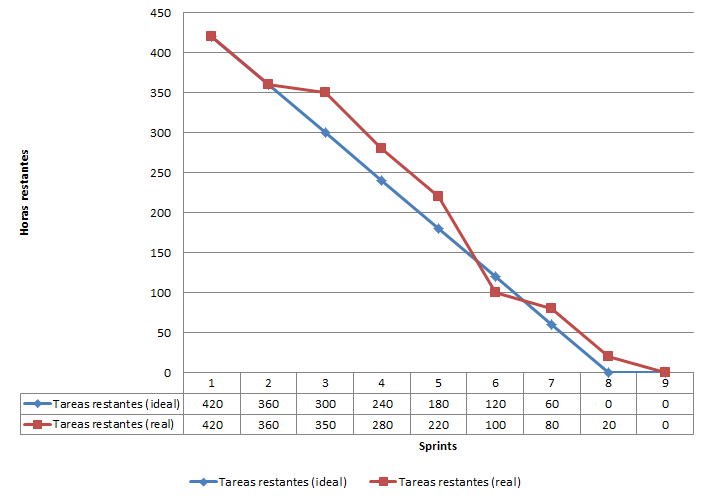
\includegraphics[width=0.7\linewidth]{./Figures/burndown.png}
\caption{Burndown}
\label{fig:burndown}
\end{figure}

En la Figura \ref{fig:burndown} se puede ver las tareas que me quedaban en cada iteraci\'on
y cual era el progreso ideal para acabarlo a tiempo. Tal y como de puede observar,
las dos l\'ineas no van ni mucho menos cerca, aunque finalmente la fecha de entrega sea muy similar.

Esto sirve para ver que aunque en algunos sprints se vaya con ``retraso", no implica que el proyecto
en general vaya con retraso.

Hay que contar como han sido realmente las cosas: tiempos, distribucion del trabajo, 
sensaciones que se han tenido al usar scrum etc. Por lo que habra que crear el
burndown para mostrar como ha sido realmente el trabajo, que nuevas tareas han surgido...

Lo complicado que es trabajar en una tecnologia que apenas conoces, ademas utilizando
librerias con escasa documentacion, en la que todo tu trabajo se basa en prueba y error
y en mirar si otras personas han tenido antes el mismo problema que tu utilizando
ademas la misma biblioteca.
    
    
    
\backmatter
    %plain, alpha, amsplain, amsalpha
    \bibliographystyle{apacite}
    \bibliography{./Bibliography/bibliografia}
    
% bibliography, glossary and index would go here.

\end{document}